\documentclass{aiaa-tc}
\usepackage{amsmath,epstopdf}
\usepackage{subfigure,morefloats}
\usepackage{caption,multirow}
\usepackage{subfigmat}
\usepackage{caption}
\usepackage{bbding}

\newcommand{\psibold}{\mbox{\boldmath$\psi$}}
\newcommand{\nablabold}{\mbox{\boldmath$\nabla$}}
\newcommand{\sigmabold}{\mbox{\boldmath$\sigma$}}
\newcommand{\Omegabold}{\mbox{\boldmath$\Omega$}}
\newcommand{\Gammabold}{\mbox{\boldmath$\Gamma$}}
\newcommand{\degr}{ ^{\circ}}
\renewcommand{\l}{\left}
\renewcommand{\r}{\right}

%List of authors:
%Manuel R. L\'opez-Morales
%Abhishek Sheshadri
%Kartikey Asthana
%Jacob Crabill
%Thomas Economon
%David Manosalvas
%Joshua Romero
%Jerry Watkins
%David Williams
%Dr. Francisco Palacios
%Prof. Antony Jameson

\title{Verification and Validation of HiFiLES: a High-Order LES unstructured solver on multi-GPU platforms}

 \author{Manuel R. L\'opez-Morales
         \thanks{Ph.D. Candidate, Department of Aeronautics and Astronautics, Stanford University, AIAA Student Member; mlopez14@stanford.edu},
            Jonathan Bull\thanks{Postdoctoral Scholar, Department of Aeronautics and Astronautics, Stanford University, AIAA Member},
            Jacob Crabill,\thanks{Ph.D. Candidates (authors in alphabetical order), Department of Aeronautics and Astronautics, AIAA Student Members},\\
            Thomas D. Economon\footnotemark[3],
            David Manosalvas\footnotemark[3],\\
            Joshua Romero\footnotemark[3],
            Abhishek Sheshadri\footnotemark[3],
            Jerry E. Watkins II\footnotemark[3],
            David Williams\thanks{CFD Engineer, Flight Sciences Division, Boeing Commercial Airplanes, AIAA Member},\\
            Francisco Palacios\thanks{Engineering Research Associate, Department of Aeronautics and Astronautics, AIAA Senior Member}, and
            Antony Jameson\thanks{Thomas V. Jones Professor of Engineering, Department of Aeronautics and Astronautics, Stanford University, AIAA Fellow} \\
           \normalsize\itshape
         Department of Aeronautics and Astronautics, Stanford University, Stanford, CA, 94305
         }


\begin{document}

\maketitle

% !TEX root = ./main.tex

\begin{abstract}
The goal of this paper is to present a verification and validation study of HiFiLES: a high-order LES solver developed in the Aerospace Computing Laboratory (ACL) at Stanford University. HiFiLES has been built on top of SD++ (Castonguay et al.) and achieves high-order spatial discretizations with the Energy-Stable Flux Reconstruction (ESFR) scheme on unstructured grids in two and three dimensions. The high parallelizability of this scheme motivates the optimization of the solver's ability to run in a multi-GPU (Graphical Processing Unit) environment.
We intend for this paper to be the main reference for HiFiLES and serve (with the previous SD++ papers) as a reference for researchers that would like to develop or implement high-order numerical schemes based on an Energy-Stable Flux Reconstruction (ESFR) approach.
\end{abstract}

%% !TEX root = ./main.tex

\section*{Nomenclature}

 \begin{tabbing}
  XXXXXXXXXXX \= \kill % first line sets tab stop

$\Omega$ \> Simulation domain \\
$\Omega_s$ \> Reference element domain \\
$\Gamma$ \> Element mapping: physical to reference domain \\
$\lambda$ \> Viscosity of medium \\
$\eta^e$ \> Bassi Rebay weighting constant \\

$c$ \> Correction function parameter \\
$f, \hat{f}^{\delta} $ \> Inviscid flux, untransformed and transformed \\
%$\hat{f}^{\delta D}$\hat{f}^{\delta I}, \hat{f}^{\delta C} $ \> Inviscid flux, discontinuous, interface, correction \\

$f_v, \hat{f_v}^{\delta} $ \> Viscous flux, untransformed and transformed \\
%$\hat{f_v}^{\delta D}, \hat{f_v}^{\delta I}, \hat{f_v}^{\delta C} $ \> Viscous flux, discontinuous, interface, correction \\

$g, g_L, g_R$ \> Correction functions, generic, left and right interfaces \\

$J$ \> Element jacobian \\

$k$ \> Degree of discontinuous solution basis \\
$L_k$ \> Legendre polynomial degree k \\
$l_k$ \> Lagrange polynomial degree k \\

$r$ \> Coordinate in reference domain \\
$r_e$ \> Bassi Rebay lifting operator \\
$t$ \> Time based on simulation units \\
$u, \hat{u}^{\delta} $ \> Solution, untransformed and transformed \\
%$\hat{u}^{\delta D}, \hat{u}^{\delta I}, \hat{u}^{\delta C} $ \> Solution flux, discontinuous, interface, correction \\
$x$ \> Coordinate in physical domain \\

 \end{tabbing}

\section{Introduction}
Low-order methods are ubiquitous in industry and academia. Regardless of the mesh quality and flow conditions, commercial \gls{cfd} packages output an answer. It is up to the informed user to decide if such answer is believable or accurate to her satisfaction. This is not so true of high-order methods: they are still sensitive to starting conditions, mesh quality, and the non-linearity of the flow, i.e. how high \gls{re} is. If any of these parameters is not chosen well, the simulation will halt prematurely and no result, not even a rough estimate, will be provided. Certainly, this is not acceptable in an industrial setting.

The \gls{lfs} filters being proposed in this chapter are an attempt at tackling the low robustness of high-order methods from the perspective of flow physics, rather than the classical frameworks of polynomial order reduction, artificial viscosity, or limiting. Very promising results have been shown by Asthana and the author~\cite{asthana2014} for 1D non-linear advection-diffusion problems and 2D inviscid high-\gls{ma} flows with quadrilateral, unstructured, coarse grids, and polynomial discretizations of up to order $8$. The present paper extends their formulation to arbitrary elements in arbitrary dimensions and shows results in high-\gls{re} flows without turbulence modeling.

It is well known that turbulent flows --which tend to be high-\gls{re}--, exhibit an energy cascade: the energy from large scales is transferred to smaller scales due to natural dissipation. In very crude terms, large vortices become ever smaller vortices until they reach dimensions proportional to the Kolmogorov length-scale~\cite{kolmogorov1962refinement}. This phenomenon is well captured by the \gls{ns} equations. Hence, a good \gls{ns} solver would see large scales become ever smaller. In general, low-order methods in grids not created for \gls{dns} introduce enough numerical dissipation that the ever shrinking scales are dissipated before they become aliased (or under-sampled).

We postulate that it is precisely this very natural energy cascade which is de-stabilizing high-order numerical methods. Because high-order methods introduce little numerical dissipation, the ever shrinking scales may not be dissipated before they become aliased: they re-appear as larger scales that, naturally, become smaller later on. This vicious cycle introduces non-physical energy into the flow until the simulation is de-stabilized. Thus, removing the small scales before they become aliased would, in theory, stabilize the solution.

\gls{lfs} filters target scales relative to the element size, as the filtering operation happens in the reference element. The smaller the element, the smaller the scale being filtered. In addition, the filters help satisfy boundary conditions. The  results presented here show that the \gls{lfs} filters can  stabilize not only high-$\Re$ flows but also moderate-$\Ma$ and low-$\Ma$ flows in coarse grids, which opens the door to using the filters as pre-conditioners or in multigrid cycles. All simulations being presented ran from start to finish without intervention.

Many stabilization schemes created for high-order methods have focused on shock-capturing. A concise review of the shock-capturing literature can be seen in Section 3.4 in~\cite{vincent2011facilitating}. An \gls{av}-based shock capturing approach that has gained popularity because of its ease of implementation and increase of robustness was suggested by Persson and Peraire~\cite{persson2006sub}. A similar approach for high-$\Re$ flows with turbulence modeling has been proposed by Nguyen et al.~\cite{nguyen2007rans}. Lodato~\cite{lodato2014structural} has used filtering in the formulation of \gls{sgs} models for \gls{les} with high-order \gls{sd} schemes. His work inspired the formulation of the filters presented here. A stabilization strategy based on optimization was suggested by Guba et al.~\cite{guba2014optimization} shows great promise. A limiter-based stabilization strategy easily implemented in \gls{dg}-type methods was proposed by Kuzmin~\cite{kuzmin2004high} and Lv et al.~\cite{lv2015entropy}.

The main reason we decided to find a stabilization strategy that could be posed as a matrix multiplication and requires a very local stencil arises from the fact that \gls{hf} performs best on \gls{gpu}s. \gls{gpu}s require a low-communication, highly-parallel implementation with organized memory accesses and homogeneous computations. Implementation of \gls{av} would have required elements adjacent to each other to share information about the \gls{av} that each requires, leading to inevitable additional inter-element communication.

 Section \ref{sec:frmethod} presented a general description of the \gls{fr} method. Section \ref{sec:extension_multiple_dimensions} showed how this scheme relies on matrix multiplications and, hence, a filter that costs two small matrix multiplications per element is ideal for \gls{fr}. Section \ref{sec:lfsfilter} describes the properties being sought in the \gls{lfs} filters and the mechanics of their implementation. Section \ref{sec:visualization} provides visualizations of the filters and their effects on a polynomial solution. Section \ref{sec:results} presents the results of 2D simulations, in unstructured coarse grids, of flows where \gls{re}$= 1e6$. This \gls{re} number was selected because of the availability of experimental data for the case of the circular cylinder and \gls{hf} had not been run at these \gls{re} numbers. In addition, Section \ref{sec:filteringEffects} shows results that isolate the effects of filtering from the effects of coarsening a grid or changing the spatial order of accuracy to demonstrate that \gls{lfs} filters preserve element-wise spectral properties.



\section{Governing Equations}
\label{sec:govEq}

\section{Numerics}
\label{sec:numerics}
\subsection{Flux Reconstruction Method}

What follows is an overview of the flux reconstruction (FR) framework. We start the discussion with the solution of the advection equation in one dimension using the FR approach to illustrate the peculiarities of the method. Then we proceed to describe the solution of the advection in two and three dimensions to show how the scheme works in triangular and tetrahedral elements. 
More details about FR and ESFR properties and derivations can be found in the articles and papers by Williams, Vincent, Castonguay, Jameson, and Huynh.

\subsubsection{Solution of the Advection Equation in One Dimension using the FR Approach}

Consider the one-dimensional conservation law
\begin{equation}
\label{eq:cons}
\frac{\partial u}{\partial t} + \frac{\partial f}{\partial x} = 0
\end{equation}

in domain $\Omega$, where $x$ is the spatial coordinate, $t$ is time, $u$ is a scalar function of $x$ and $t$, and $f$ is a scalar function of $u$. Note that letting $f = f(u,\frac{\partial u}{\partial x})$, Equation\ref{eq:cons} becomes a model of the Navier-Stokes equations.

Let us partition the domain $\Omega = [x_1,x_{N+1})$ into $N$ non-overlapping elements with 
interfaces at $x_1<x_2<...<x_{N+1}$. Then,
$$
\Omega = \bigcup^N_{n=1} \Omega_n
$$
and $\Omega_n = [x_n,x_{n+1})$ for $n = 1,...,N$.

To simplify the implementation, let us map each of the physical elements $\Omega_n$ to a standard 
element $\Omega_s=[-1,1)$ with the function $\Theta_n(\xi)$, where
$$
x = \Theta_n(\xi) = \l( \frac{1-\xi}{2} \r) x_n + \l(\frac{1+\xi}{2}\r) x_{n+1} 
$$

With this mapping, the evolution of $u$ within each $\Omega_n$ can be determined with the following 
transformed advection equation
$$
\frac{\partial \hat{u}}{\partial t} + \frac{\partial \hat{f}}{\partial \xi} = 0
$$
where
$$
\hat{u} = J_n u(\Theta_n(\xi),t) \text{ in } \Omega_n
$$
$$
\hat{f} = f(\Theta_n(\xi),t) \text{ in } \Omega_n
$$

Now, introduce polynomial approximations $\hat{u}^\delta, \hat{f}^\delta$ to 
the exact values $\hat{u},\hat{f}$, respectively. Using piecewise polynomials of degree $p$ as 
approximations, we can write
$$
\hat{u}^\delta = \sum_{i=1}^{N_s} \hat{u}_i^\delta l_i(\xi)
$$
$$
\hat{f}^\delta = \sum_{i=1}^{N_s} \hat{f}_i^\delta l_i(\xi)
$$
where $N_s$ is the number of solution points, $\hat{u}_i^\delta$ is the current value of the 
solution approximation function at the $i^\text{th}$ solution point in the reference element, 
$\hat{f}_i^\delta$ is the current value of the flux approximation function at the $i^\text{th}$ 
solution point in the reference element, $l_i$ is the Lagrange polynomial equal to $1$ at the 
$i^\text{th}$ solution point and $0$ in the others, and $\delta$ signals that the function is an 
approximation.

Note that the piecewise polynomials may not be continuous (or $c_0$) accross the interfaces. In the 
Flux Reconstruction approach, the flux used in the time advancement of the solution is made $c_0$ 
by introducing flux correction functions. To this end, in the general non-linear advection case, it 
is necessary to first make the solution $c_0$.

This can be done by finding interface values at each element and then correcting the 
solution. Let $\hat{u}_L^{\delta I}$ and $\hat{u}_R^{\delta I}$ be the interface values at left and right 
boundaries of each element, respectively. Then, select solution correction functions $g_L$ and 
$g_R$ such 
that
$$
g_L(-1) = 1 \; g_L(1) = 0
$$
$$
g_R(-1) = 0 \; g_R(1) = 1
$$
and let
$$
\hat{u}^c = \hat{u}^\delta + (\hat{u}^{\delta I}_L - \hat{u}^\delta_L) g_L + (\hat{u}^{\delta I}_R 
- \hat{u}^\delta_R) g_R
$$
where superscript $c$ denotes the function is corrected, and $\hat{u}^\delta_L$, $\hat{u}^\delta_R$ 
represent the solution approximation evaluated at the left and right boundaries.

We can proceed in a similar fashion to correct the flux to obtain
$$
\hat{f}^c = \hat{f}^\delta + (\hat{f}^{\delta I}_L - \hat{f}^\delta_L) h_L + (\hat{f}^{\delta I}_R 
- \hat{f}^\delta_R) h_R
$$
where $h_R$ and $h_L$ are right and left flux correction functions satisfying the same boundary 
conditions as $g_R$ and $g_L$, respectively.

The solution can then be advanced at each solution point. In semi-discrete form, this is
$$
\frac{d \hat{u}_i^\delta}{d t} = - \frac{\partial \hat{f}^c}{\partial \xi}(\xi_i)
$$

The FR scheme can be made stable by selecting special types of correction functions.

%The final paper, for completeness, will include a description of the Flux Reconstruction\cite{vincent2011new} approach and the reasoning behind using the Energy-Stable version. A thorough description of the steps taken in the calculation of the residual for the 3D NS Equations will be included.


\subsection{Unstructured Mesh Treatment}
Mention developments in squares (tensor products of linear scheme), triangles\cite{castonguay2012new,williams2013tri}, tetrahedra\cite{williams2013tet}, prisms (tensor product of linear with triangular schemes), and hexahedra (tensor products of linear scheme).

\subsection{Time Stepping and p-multigrid}
Explicit RK4 with ability to use multigrid\cite{fidkowski2005p} and dual time-stepping\cite{Jameson1991DualTime} for implicit time advancement.

%\subsection{Stabilization Techniques}

\subsection{Large Eddy Simulation Models}
SGS Models: Smagorinsky\cite{smagorinsky1963}, WALE\cite{nicoud1999}, WALE-similarity\cite{lodato2009}, SVV\cite{karamanos2000}.
Filters: Vasilyev\cite{vasilyev1998,vasilyev2001}, discrete Gaussian\cite{lodato2012b}, Modal Vandermonde\cite{blackburn2003}.

\subsection{Computing Architecture and Scalability}
%The final paper will include a description of how HiFiLES is designed for a multi-GPU environment. Studies performed without filtering or SGS modeling in \cite{castonguay2011}. 
The Hi-FiLES code has been designed to work on multi-CPU as well as multi-CPU-GPU platforms. The Flux Reconstruction method in its current form with explicit time-stepping has a great potential for parallelization. Since the solution points are not explicitly shared between elements, most of the computations are element-local enabling an efficient use of shared memory on GPUs. Also, several computations are independent for each solution point and the highly parallelizable nature of GPUs becomes very useful. A detailed description of the paralleization of the FR method, along with scalability and performance analysis has been performed in \cite{castonguay2011}.

\subsection{Shock capturing and Stabilization Models}
Currently, we have adapted Persson and Peraire's method \cite{Persson06} for shock detection and capturing. The method works well for inviscid flow cases and compressible flows upto a Mach number of 2 have been tried and tested. However the method requires fine-tuning of parameters for each problem and we are currently working on a new method which is more robust. Persson and Peraire have used this shock capturing tool as a stabilization method as well in their turbulence calculations and we plan to test this and present results for inviscid and viscous cases in the final draft. Here we show a few inviscid results for the case of M = 1.6 where we illustrate the ability to detect shocks and add dissipation in a local manner in the form of artificial viscosity in order to capture the shock in a fine manner and avoid the loss of accuracy away from the shock.    

\begin{figure}[h] \tt
\centering
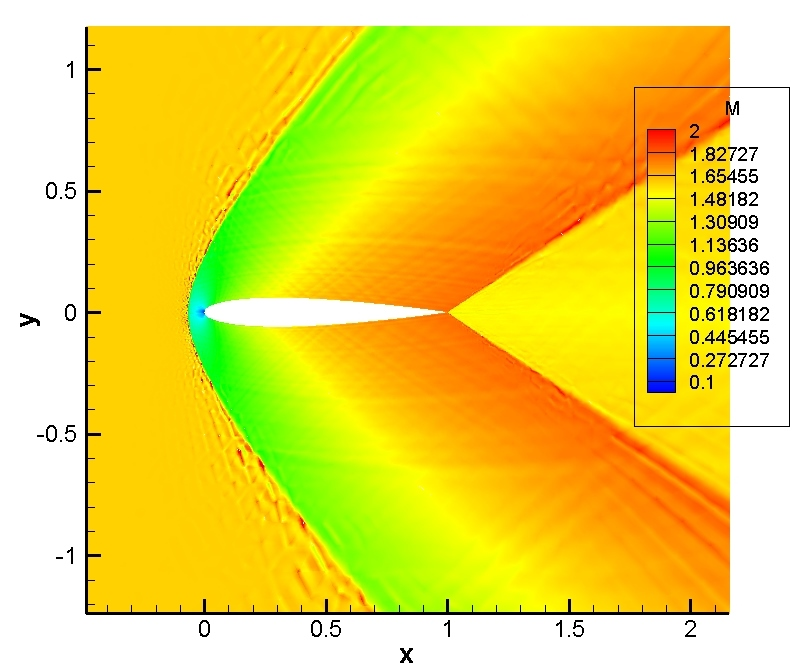
\includegraphics[angle=0, scale = 0.55]{./figures/M1pt6order3-inv-720ktime-mach.jpg} \\
\caption{Mach contours for inviscid flow over Naca0012 at M = 1.6 and AoA = $0^{\circ} $}
\label{fig:inv_mach}
\end{figure}

\begin{figure}
\centering
\begin{minipage}[t]{.5\textwidth}
  \centering
  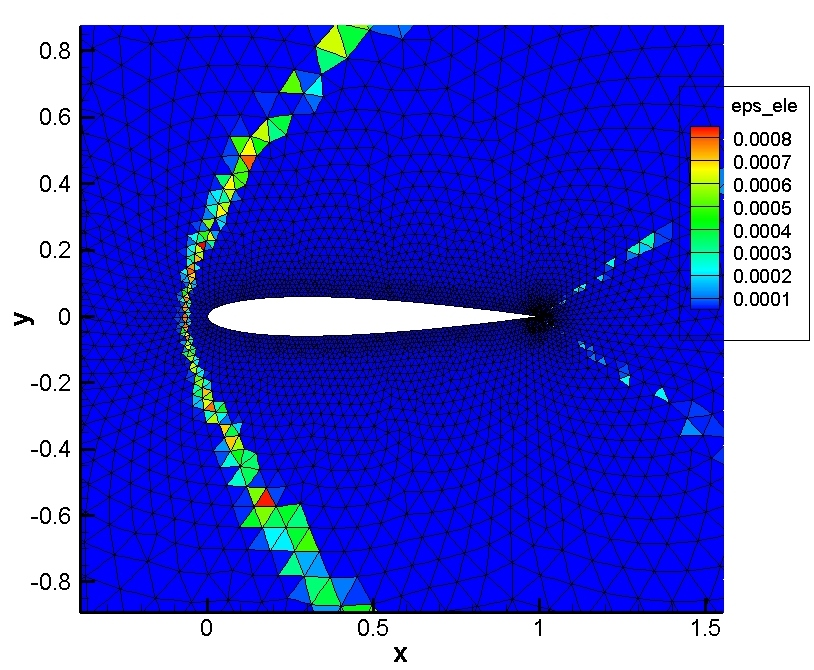
\includegraphics[width=.85\linewidth]{./figures/M1pt6-inv-av-ele-mesh}
  \captionof{figure}{Element-wise AV co-efficients (case 1)}
  \label{fig:AV-ele}
\end{minipage}%
\begin{minipage}[t]{.5\textwidth}
  \centering
  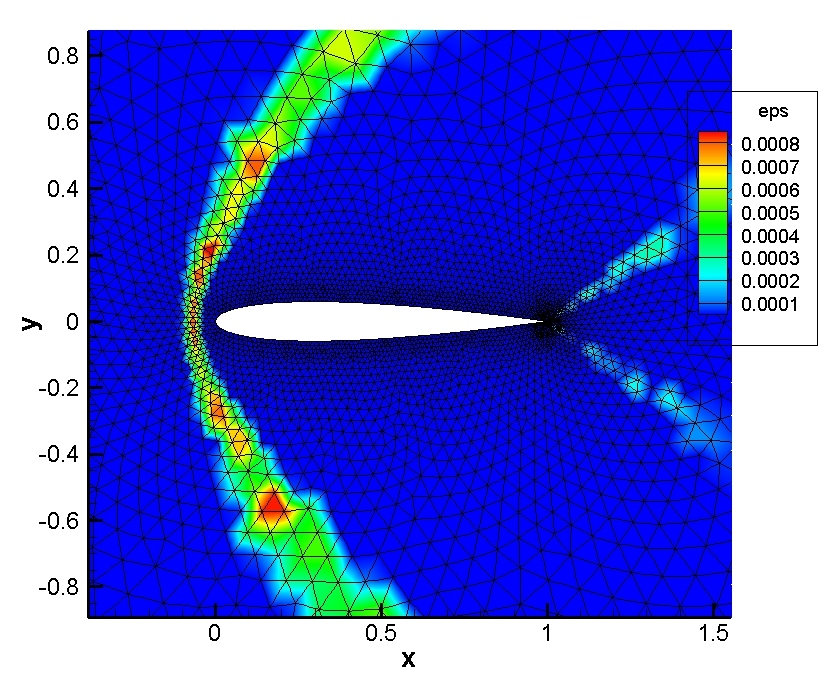
\includegraphics[width=.85\linewidth]{./figures/M1pt6-inv-av-mesh}
  \captionof{figure}{AV co-efficients with continuity enforcement}
  \label{fig:AV-cont}
\end{minipage}
\end{figure} 



% !TEX root = ../thesis.tex

\section{Verification and Validation}

\label{sec:verification}

% Manufactured solutions
% !TEX root = ../thesis.tex
\graphicspath{{figures_manufactured/}}% Set graphics path location


\subsection{Method of Manufactured Solutions}

This section describes the test of \gls{hf}'s spatial order of accuracy using the \gls{mms} in 2D and 3D for viscous flows. As shown by Salari et. al~\cite{salari2000code}, the \gls{mms} test rigorously assesses the correctness of implementation of a solver of \gls{pde}s. Simplex elements are crucial for simulations in unstructured meshes and have a more complex implementation than squares and hexahedra. As a result, we perform the \gls{mms} test in grids using simplex elements.

The \gls{mms} test for \gls{ns} solvers requires checking the solver's solution against an exact solution. Such exact solution can be chosen arbitrarily. The \gls{ns} equations can be satisfied with this arbitrary solution by including a time-dependent source term in the equations. Then, we solve

\begin{equation}
\frac{\partial U}{\partial t} +  \nabla \cdot {\bf F} = S
\end{equation}

For the following tests, we selected a smooth exact solution, so aliasing does not pollute the results. We picked

\begin{equation}\label{eq:NSwithSource}
\begin{split}
U_{2D} = \l(
\begin{tabular}{c}
$\sin{(k(x+y) - \omega t)} + a$\\
$\sin{(k(x+y) - \omega t)} + a$\\
$\sin{(k(x+y) - \omega t)} + a$\\
$(\sin{(k(x+y) - \omega t)} + a)^2$
\end{tabular}
\r) \\
U_{3D} = \l(
\begin{tabular}{c}
$\sin{(k(x+y+z) - \omega t)} + a$\\
$\sin{(k(x+y+z) - \omega t)} + a$\\
$\sin{(k(x+y+z) - \omega t)} + a$\\
$\sin{(k(x+y+z) - \omega t)} + a$\\
$(\sin{(k(x+y+z) - \omega t)} + a)^2$
\end{tabular}
\r)
\end{split}
\end{equation}

To find the value of $S$, we plug the values of our selected $U$ into the left-hand side of Equation~\eqref{eq:NSwithSource} and simplify. The resulting expression is $S$. 
We let \gls{pr}$=0.72, \gamma = 1.4, k = \pi, \omega = \pi, a = 3.0$ and $\mu = 0.001$.

The meshes used have dimensions $[-1,1] \times [-1,1]$ in 2D and $[-1,1] \times [-1,1] \times [-1,1]$ in 3D. Periodic boundary conditions were applied on the boundaries of the square and cube domains. Uniform square and cubic meshes were created and then each element was subdivided into triangles or tetrahedra. Two triangles were created from each square, and six tetrahedra were created from each cube. Consequently, in 2D a $N \times N$ mesh contains $2N^2$ triangles, and in 3D a $N \times N \times N$ mesh contains $6N^3$ tetrahedra. 


In 3D, the time step was $1$e$-4$ seconds and 10 seconds of flow were simulated. In 2D, the time step was $1$e$-6$ seconds and 1 second of flow was simulated. The time-stepping scheme used was the low-storage, $4^\text{th}$ order accurate \gls{rk45} method. 


% !TEX root = ../thesis.tex
\begin{table}[htbp]
\centering
\begin{tabular}{ c c c c c c c} 
  
 \specialcell{Polynomial\vspace{0.2cm}\\ Order} & Mesh: & 2x2x2 & 4x4x4 & 8x8x8 & 16x16x16 & \specialcell{Overall Order \vspace{0.2cm}\\ of Accuracy} \\ 
 \hline 
 \multirow{2}{*}{$p = 1$} & $L_2$ error & 5.76e-01 & 1.35e-01 & 3.22e-02 & 7.90e-03 &   \\ 
  
   & $\mathcal{O}(L_2)$ &   & 2.10 & 2.06 & 2.03 & 2.06 \\ 
 \hline 
 \multirow{2}{*}{$p = 2$} & $L_2$ error & 4.09e-01 & 5.52e-02 & 6.87e-03 & 8.53e-04 &   \\ 
  
   & $\mathcal{O}(L_2)$ &   & 2.89 & 3.01 & 3.01 & 2.97 \\ 
 \hline 
 \multirow{2}{*}{$p = 3$} & $L_2$ error & 9.77e-02 & 5.97e-03 & 3.78e-04 &   &   \\ 
  
   & $\mathcal{O}(L_2)$ &   & 4.03 & 3.98 &   & 4.01 \\ 
 \hline 
 \multirow{2}{*}{$p = 4$} & $L_2$ error & 1.12e-02 & 6.39e-04 & 2.07e-05 &   &   \\ 
  
   & $\mathcal{O}(L_2)$ &   & 4.13 & 4.95 &   & 4.54 \\ 
 \hline 
 \multirow{2}{*}{$p = 5$} & $L_2$ error & 1.53e-01 & 5.08e-03 & 6.92e-05 &   &   \\ 
  
   & $\mathcal{O}(L_2)$ &   & 4.91 & 6.20 &   & 5.55 \\ 
 \hline 
 \end{tabular}
\caption{Accuracy of \gls{hf} for NS equations with source term in tetrahedral meshes at $t = 10$. $L_2$ error is the $L_2$-norm of the error in the energy field: $\rho e$}
\label{table:tetsError1} 
 \end{table}

% !TEX root = ../thesis.tex
\begin{table}[htbp]
\centering
\begin{tabular}{ c c c c c c c} 
  
 \specialcell{Polynomial\vspace{0.2cm}\\ Order}  & Mesh: & 2x2x2 & 4x4x4 & 8x8x8 & 16x16x16 & \specialcell{Overall Order \vspace{0.2cm}\\ of Accuracy} \\ 
 \hline 
 \multirow{2}{*}{$p = 1$} & $L_2$ error & 1.98e+01 & 9.57e+00 & 4.55e+00 & 2.19e+00 &   \\ 
  
   & $\mathcal{O}(L_2)$ &   & 1.05 & 1.07 & 1.06 & 1.06 \\ 
 \hline 
 \multirow{2}{*}{$p = 2$} & $L_2$ error & 1.17e+01 & 2.98e+00 & 7.10e-01 & 1.71e-01 &   \\ 
  
   & $\mathcal{O}(L_2)$ &   & 1.97 & 2.07 & 2.06 & 2.03 \\ 
 \hline 
 \multirow{2}{*}{$p = 3$} & $L_2$ error & 3.17e+00 & 3.81e-01 & 4.73e-02 &   &   \\ 
  
   & $\mathcal{O}(L_2)$ &   & 3.06 & 3.01 &   & 3.03 \\ 
 \hline 
 \multirow{2}{*}{$p = 4$} & $L_2$ error & 5.21e-01 & 4.27e-02 & 2.69e-03 &   &   \\ 
  
   & $\mathcal{O}(L_2)$ &   & 3.61 & 3.99 &   & 3.80 \\ 
 \hline 
 \multirow{2}{*}{$p = 5$} & $L_2$ error & 3.20e+00 & 1.88e-01 & 4.79e-03 &   &   \\ 
  
   & $\mathcal{O}(L_2)$ &   & 4.09 & 5.29 &   & 4.69 \\ 
 \hline 
 \end{tabular}
\caption{Accuracy of \gls{hf} for NS equations with source term in tetrahedral meshes at $t = 10$. $L_2$ error is the $L_2$-norm of the error in the gradient of the energy field:$\frac{\partial}{\partial x_i} (\rho e)$}
\label{table:tetsError2} 
 \end{table}

% !TEX root = ../thesis.tex

\begin{table}[htbp]

%\centering
  \hspace{-1.1cm}
\begin{tabular}{ c c c c c c c c} 

 \specialcell{Polynomial\vspace{0.2cm}\\ Order}  & Mesh: & 4x4 & 8x8 & 16x16 & 32x32 & 64x64 & \specialcell{Overall Order \vspace{0.2cm}\\ of Accuracy}  \\ 
 \hline 
 \multirow{2}{*}{$p = 1$} & $L_2$ error & 7.92e-01 & 1.84e-01 & 4.36e-02 & 1.07e-02 & 2.68e-03 &   \\ 
  
   & $\mathcal{O}(L_2)$ &   & 2.10 & 2.08 & 2.03 & 2.00 & 2.05 \\ 
 \hline 
 \multirow{2}{*}{$p = 2$} & $L_2$ error & 1.29e-01 & 1.61e-02 & 1.95e-03 & 2.33e-04 & 2.86e-05 &   \\ 
  
   & $\mathcal{O}(L_2)$ &   & 3.00 & 3.05 & 3.06 & 3.03 & 3.04 \\ 
 \hline 
 \multirow{2}{*}{$p = 3$} & $L_2$ error & 1.01e-02 & 9.25e-04 & 5.71e-05 & 3.65e-06 & 2.35e-07 &   \\ 
  
   & $\mathcal{O}(L_2)$ &   & 3.45 & 4.02 & 3.97 & 3.96 & 3.88 \\ 
 \hline 
 \multirow{2}{*}{$p = 4$} & $L_2$ error & 2.60e-03 & 6.33e-05 & 2.00e-06 & 6.49e-08 & 3.62e-09 &   \\ 
  
   & $\mathcal{O}(L_2)$ &   & 5.36 & 4.98 & 4.95 & 4.16 & 4.88 \\ 
 \hline 
 \multirow{2}{*}{$p = 5$} & $L_2$ error & 7.15e-05 & 3.87e-06 & 6.31e-08 &   &   &   \\ 
  
   & $\mathcal{O}(L_2)$ &   & 4.21 & 5.94 &   &   & 5.07 \\ 
 \hline 
 \end{tabular}
\caption{Accuracy of \gls{hf} for NS equations with source term in triangular meshes at $t = 1$. $L_2$ error is the $L_2$-norm of the error in the energy field: $\rho e$}
\label{table:trisError1} 
 \end{table}

% !TEX root = ../thesis.tex
\hspace{-1.cm}
\begin{table}[htbp]
  \hspace{-1.2cm}
\begin{tabular}{ c c c c c c c c} 
  
 \specialcell{Polynomial\vspace{0.2cm}\\ Order} & Mesh: & 4x4 & 8x8 & 16x16 & 32x32 & 64x64 & \specialcell{Overall Order \vspace{0.2cm}\\ of Accuracy} \\ 
 \hline 
 \multirow{2}{*}{$p = 1$} & $L_2$ error & 1.61e+01 & 8.31e+00 & 3.81e+00 & 1.71e+00 & 7.84e-01 &   \\ 
  
   & $\mathcal{O}(L_2)$ &   & 0.96 & 1.12 & 1.15 & 1.13 & 1.10 \\ 
 \hline 
 \multirow{2}{*}{$p = 2$} & $L_2$ error & 4.05e+00 & 8.16e-01 & 1.90e-01 & 4.54e-02 & 1.11e-02 &   \\ 
  
   & $\mathcal{O}(L_2)$ &   & 2.31 & 2.11 & 2.06 & 2.04 & 2.12 \\ 
 \hline 
 \multirow{2}{*}{$p = 3$} & $L_2$ error & 4.71e-01 & 6.39e-02 & 7.03e-03 & 7.75e-04 & 8.84e-05 &   \\ 
  
   & $\mathcal{O}(L_2)$ &   & 2.88 & 3.18 & 3.18 & 3.13 & 3.11 \\ 
 \hline 
 \multirow{2}{*}{$p = 4$} & $L_2$ error & 1.01e-01 & 4.30e-03 & 2.31e-04 & 1.41e-05 & 5.27e-06 &   \\ 
  
   & $\mathcal{O}(L_2)$ &   & 4.56 & 4.22 & 4.04 & 1.42 & 3.67 \\ 
 \hline 
 \multirow{2}{*}{$p = 5$} & $L_2$ error & 5.04e-03 & 2.50e-04 & 7.80e-06 &   &   &   \\ 
  
   & $\mathcal{O}(L_2)$ &   & 4.33 & 5.00 &   &   & 4.67 \\ 
 \hline 
 \end{tabular}
\caption{Accuracy of \gls{hf} for NS equations with source term in triangular meshes at $t = 1$. $L_2$ error is the $L_2$-norm of the error in the gradient of the energy field:$\frac{\partial}{\partial x_i} (\rho e)$}
\label{table:trisError2} 
 \end{table}


Tables \eqref{table:trisError1} and \eqref{table:tetsError1} show the spatial order of accuracy achieved when calculating the energy fields $\rho e$ in 2D and 3D, respectively. Tables \eqref{table:trisError2} and \eqref{table:tetsError2} show the order of accuracy for the gradient of the energy field $\frac{\partial }{\partial x_i}(\rho e)$ in 2D and 3D, respectively. Because of the exact solutions that were picked, the exact values of the gradients of $\rho e$ in the $x,y,z$ directions are equal.

As expected\cite{hesthaven2007nodal}, the order of accuracy of the solution is $p+1$ and the order of accuracy of the gradient of the solution is $p$, where $p$ is the order of the polynomial used to approximate the solution fields. In the fifth order simulations, the relatively large time step introduces errors larger than the spatial discretization errors. Hence we observe sub-optimal orders of convergence in the coarsest meshes.

%\begin{figure}
%\centering
%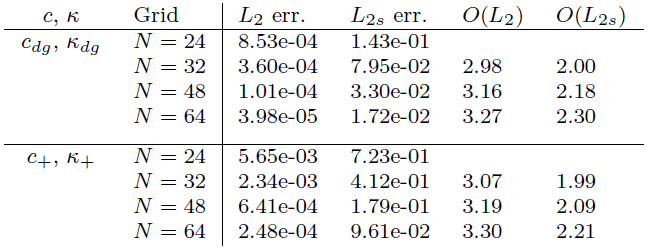
\includegraphics[height=35mm]{table_917} \\
%\caption{Accuracy of ESFR schemes for flow generated by a time-dependent source term on triangular grids, for the case of $p = 2$. The inviscid and viscous numerical fluxes were computed using a Rusanov flux with $\lambda = 1$ and a LDG flux with $\tau = 0.1$ and $\beta = \pm 0.5n$.}
%\label{fig:table_917}
%\end{figure}
%
%\begin{figure}
%\centering
%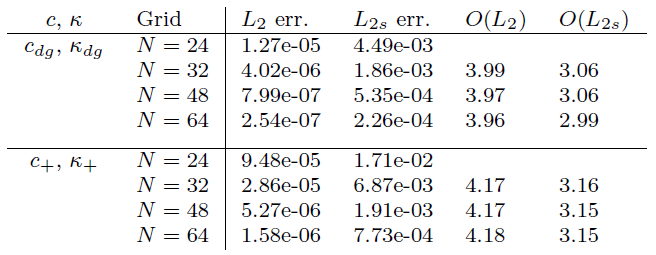
\includegraphics[height=35mm]{table_918} \\
%\caption{Accuracy of ESFR schemes for flow generated by a time-dependent source term on triangular grids, for the case of $p = 3$. The inviscid and viscous numerical fluxes were computed using a Rusanov flux with $\lambda = 1$ and a LDG flux with $\tau = 0.1$ and $\beta = \pm 0.5n$.}
%\label{fig:table_918}
%\end{figure}
%
%\begin{figure}
%\centering
%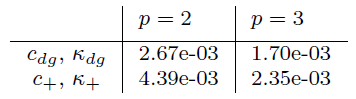
\includegraphics[height=20mm]{table_919} \\
%\caption{Explicit time-step limits ($\Delta t_{max}$) of ESFR schemes for flow generated by a time-dependent source term on the triangular grid with $\tilde{N} = 48$, for the cases of $p = 2$ and $3$. The inviscid and viscous numerical fluxes were computed using a Rusanov flux with $\lambda = 1$ and a LDG flux with $\tau = 0.1$ and $\beta = \pm 0.5n$.}
%\label{fig:table_919}
%\end{figure}
%
%\begin{figure}
%\centering
%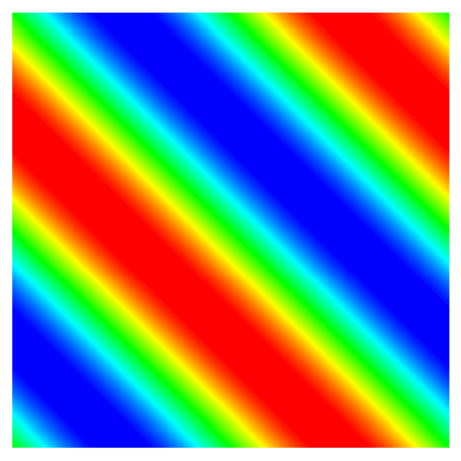
\includegraphics[height=60mm]{figure_912} \\
%\caption{Contours of energy obtained using the ESFR scheme with $c = c_+$ and $\kappa = \kappa_+$ on the triangular grid with $\tilde{N} = 32$ for the case of $p = 3$. The inviscid and viscous numerical fluxes were computed using a Rusanov flux with $\lambda = 1$ and a LDG flux with $\tau = 0.1$ and $\beta = \pm 0.5n$.}
%\label{fig:figure_912}
%\end{figure}
%
%\begin{figure}
%\centering
%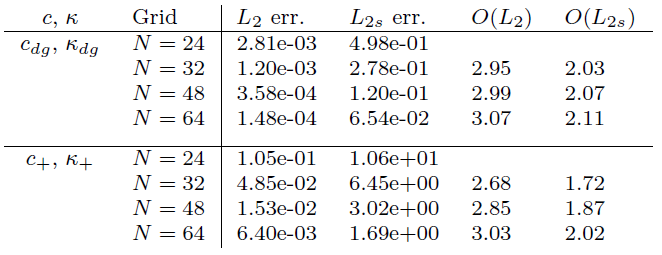
\includegraphics[height=35mm]{table_920} \\
%\caption{Accuracy of ESFR schemes for flow generated by a time-dependent source term on tetrahedral grids, for the case of $p = 2$. The inviscid and viscous numerical fluxes were computed using a Rusanov flux with $\lambda = 1$ and a LDG flux with $\tau = 0.1$ and $\beta = \pm 0.5n$.}
%\label{fig:table_920}
%\end{figure}
%
%\begin{figure}
%\centering
%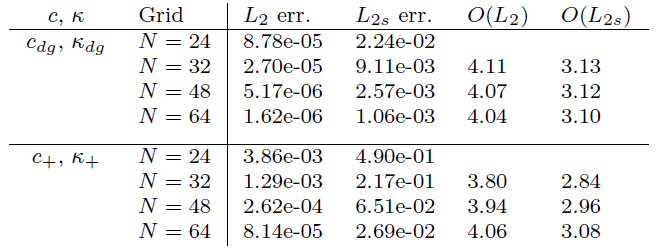
\includegraphics[height=30mm]{table_921} \\
%\caption{Accuracy of ESFR schemes for flow generated by a time-dependent source term on tetrahedral grids, for the case of $p = 3$. The inviscid and viscous numerical fluxes were computed using a Rusanov flux with $\lambda = 1$ and a LDG flux with $\tau = 0.1$ and $\beta = \pm 0.5n$.}
%\label{fig:table_921}
%\end{figure}
%
%\begin{figure}
%\centering
%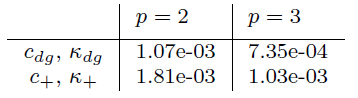
\includegraphics[height=15mm]{table_922} \\
%\caption{Explicit time-step limits ($\Delta t_{max}$) of ESFR schemes for flow generated by a time-dependent source term on the triangular grid with $\tilde{N} = 48$, for the cases of $p = 2 and 3$. The inviscid and viscous numerical fluxes were computed using a Rusanov flux with $\lambda = 1$ and a LDG flux with $\tau = 0.1$ and $\beta = \pm 0.5n$.}
%\label{fig:table_922}
%\end{figure}
%
%\newpage
%\begin{figure}
%\centering
%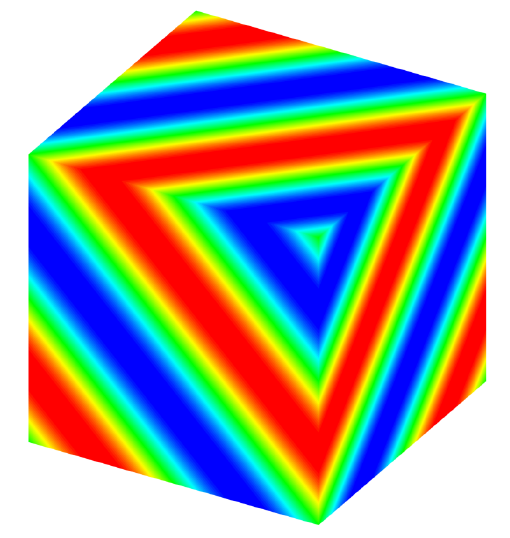
\includegraphics[height=60mm]{figure_913} \\
%\caption{Contours of energy obtained using the ESFR scheme with $c = c_+$ and $\kappa = \kappa_+$ on the tetrahedral grid with $\tilde{N} = 32$ for the case of $p = 3$. The inviscid and viscous numerical fluxes were computed using a Rusanov flux with $\lambda = 1$ and a LDG flux with $\tau = 0.1$ and $\beta = \pm 0.5n$.}
%\label{fig:figure_913}
%\end{figure}


% Flat plate
% !TEX root = ../thesis.tex
\graphicspath{{\aiaadir /figures_flatplate/}}% Set graphics path location

\subsection{Subsonic laminar flat-plate}

Computations of the flow over a subsonic flat-plate have been performed and validated against the Blasius' solution for laminar boundary layer. The flow conditions are \gls{ma} $0.5$, 0$\degr$ angle of attack and \gls{re} $1\cdot10^6$ based on the plate length. The governing equations are the 2D \gls{ns} equations with constant ratio of specific heats of $1.4$, Prandtl number of $0.72$ and constant dynamic viscosity of $1.827\cdot 10^{-5} Pa \cdot s$.

\begin{center} 
    \begin{tabular}{l*{7}{c}r}
    Mesh & First cell height & \specialcell{\# of cells in \vspace{0.2cm}\\boundary layer} & $p_3$ & $p_4$ & $p_5$ & $p_6$ \\ \hline
    Mesh a0 (140 = 14x10) & 0.00075 & 2 & $\times$ & $\times$ & $\times$ & \Checkmark \\ \hline
    Mesh a1 (560 = 28x20) & 0.000375 & 4 &  $\times$ & $\times$ & \Checkmark & \Checkmark \\ \hline
    Mesh a2 (2240 = 56x40) & 0.0001875 & 8 & $\times$ & \Checkmark & \Checkmark & \Checkmark \\ \hline
    Mesh a3 (8960 = 112x80) & 0.0000935 & 16 & \Checkmark & \Checkmark & \Checkmark & \Checkmark \\
    \hline
    \end{tabular} 
      \captionof{table}{\gls{hf} convergence using different grids and polynomial order. $\times$ / \Checkmark indicates not converged/converged resp.} \label{tab:convergence} 
\end{center}

The objective of this study is to determine the minimum number of elements and the order of polynomial required to converge the flat-plate simulation using \gls{hf}. Four different numerical grids have been used in this study (2, 4, 8, 16 elements inside the boundary layer) and four polynomial orders ($p_3$--$p_6$). The results, summarized in Table \ref{tab:convergence}, show that a minimum number of elements is needed in the boundary layer depending on the polynomial order to obtain satisfactory convergence (free from inter-element jumps).

\begin{figure}
\begin{center}
\begin{minipage}[t]{0.48\columnwidth}
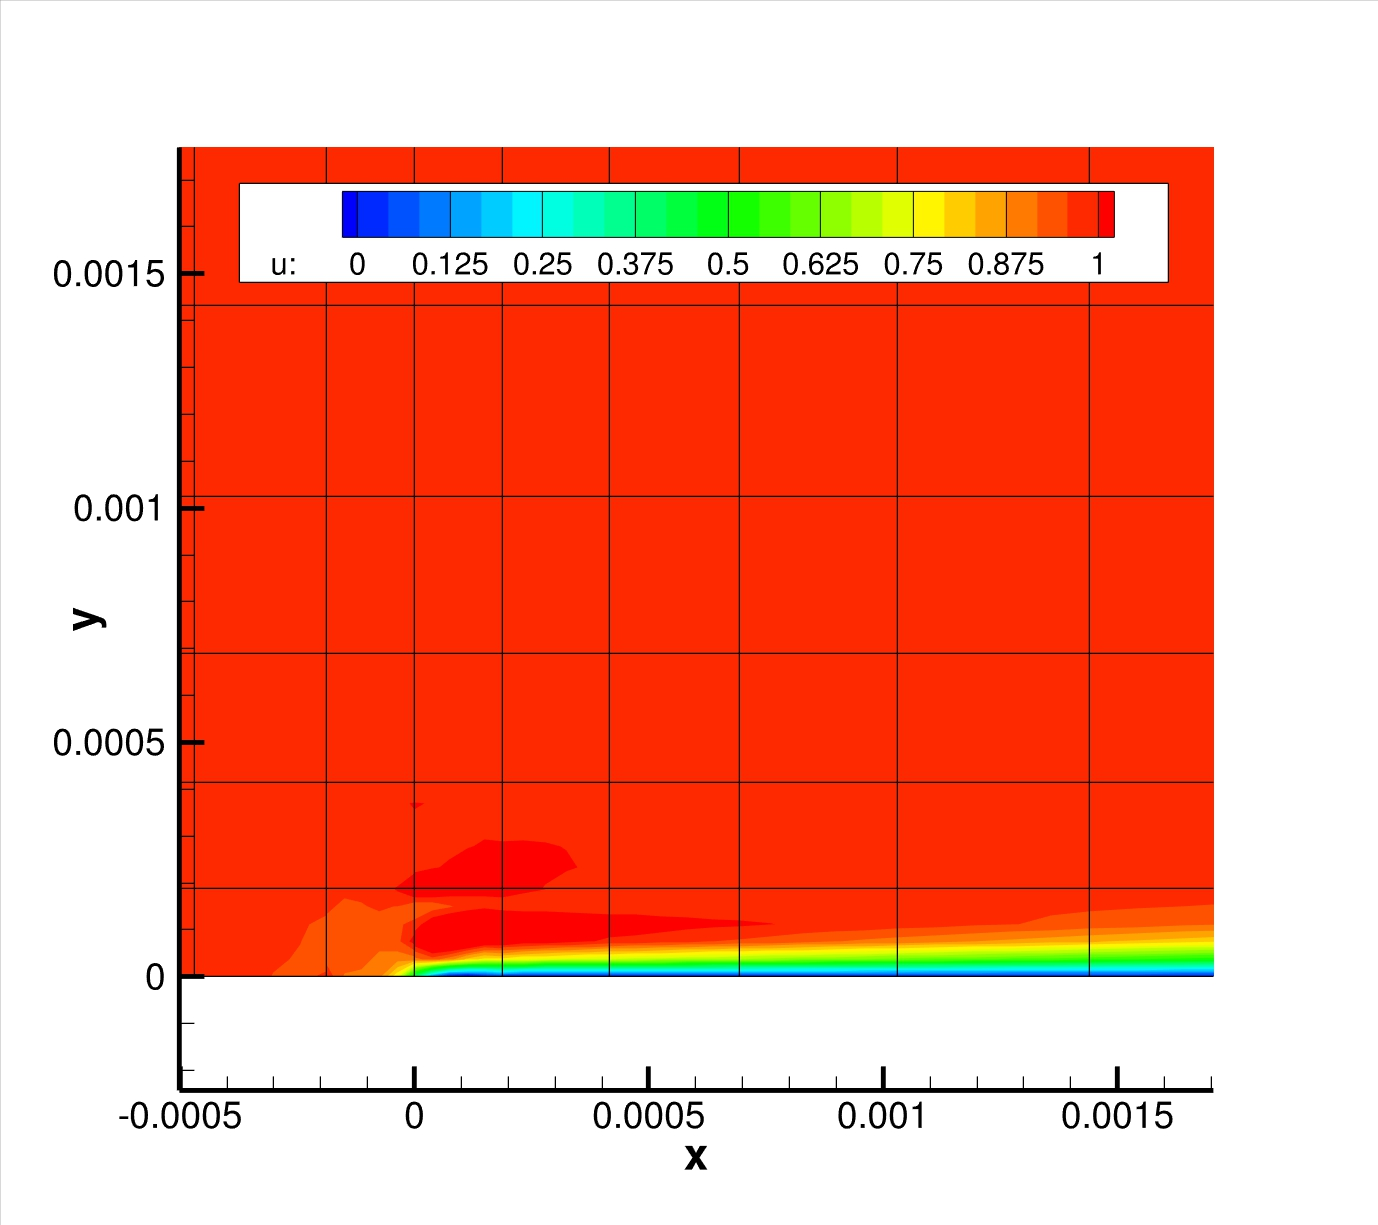
\includegraphics[width = \textwidth,clip=]{LeadingEdge.jpg}
\caption{Detail of the flat-plate leading edge (x=0.0, mesh a2).}
\label{fig:LeagingEdge}
\end{minipage}
\hfill
\begin{minipage}[t]{0.48\columnwidth}
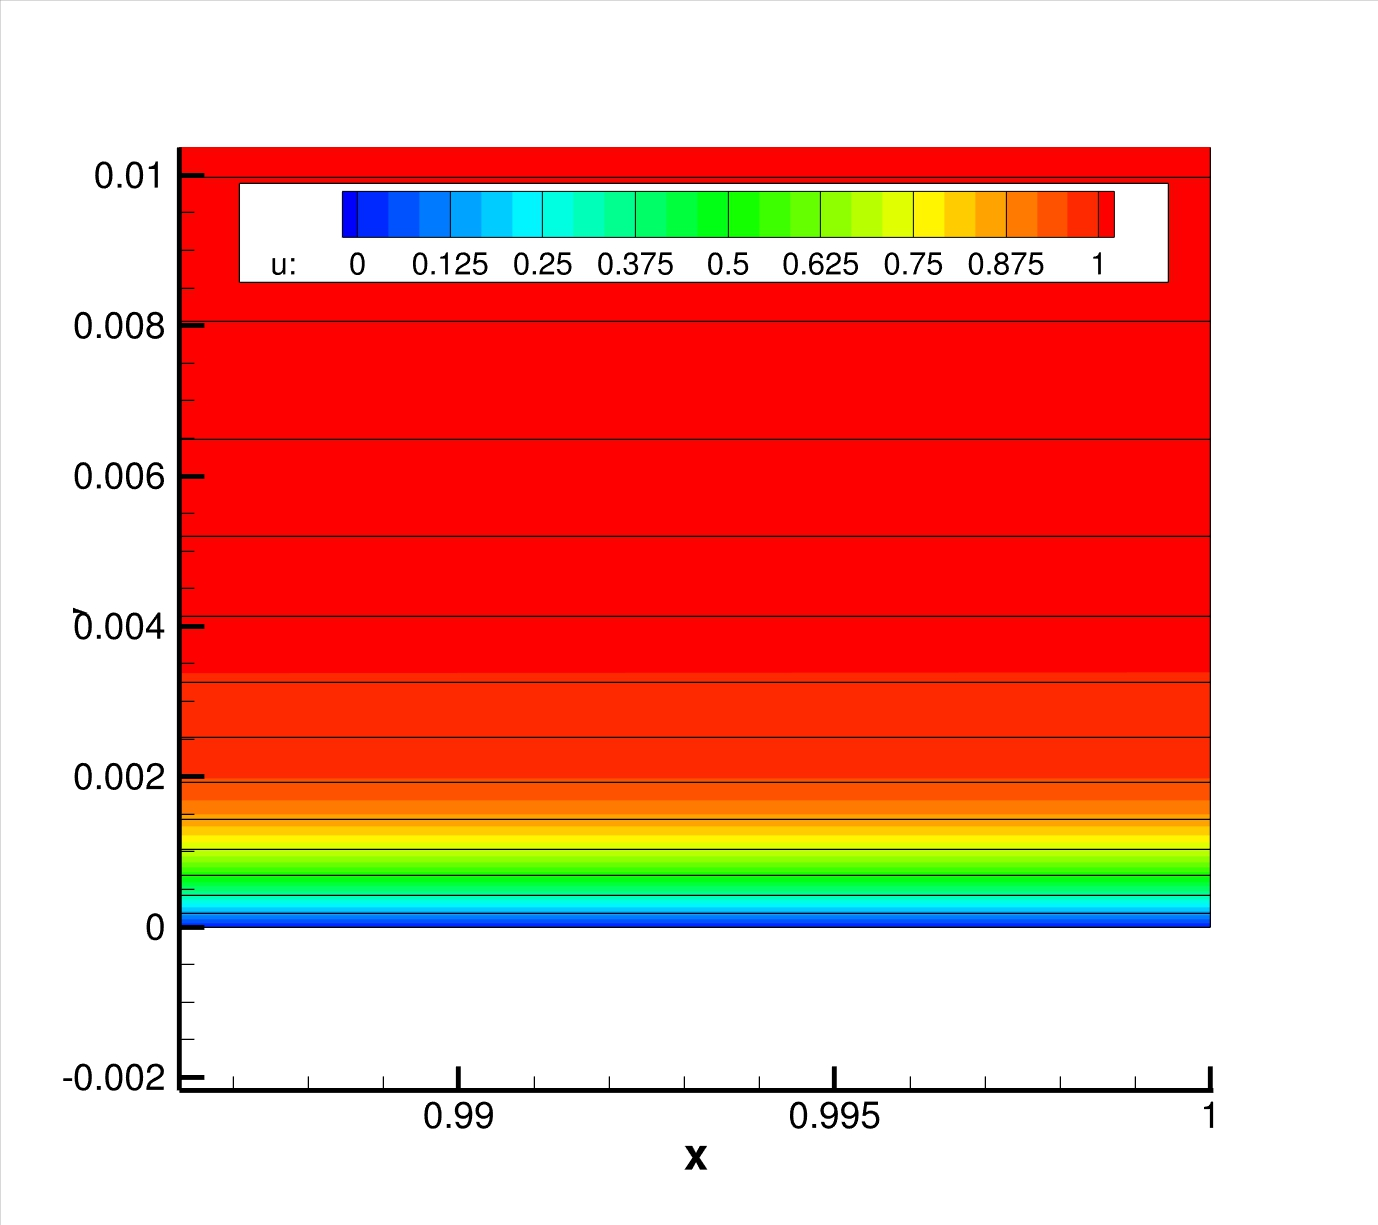
\includegraphics[width = \textwidth,clip=] {EndPlate.jpg}
\caption{Flow solution at the end of the flat-plate (x=1.0, mesh a2).}
\label{fig:TrailingEdge}
\end{minipage}
\end{center}
\end{figure}

The results are compared with the Blasius' solution for laminar boundary layer with satisfactory results, and some details of the solutions are presented in Fig. \ref{fig:LeagingEdge} (leading edge), and Fig. \ref{fig:TrailingEdge} (end of the flat-plate). It is important to note that in this particular case (mesh a2) the flat-plate boundary layer is captured using 8 elements, while in a second order solver it would be necessary of the order of ~30 elements inside the boundary layer.

\begin{figure}
\begin{center}
\begin{minipage}[t]{0.48\columnwidth}
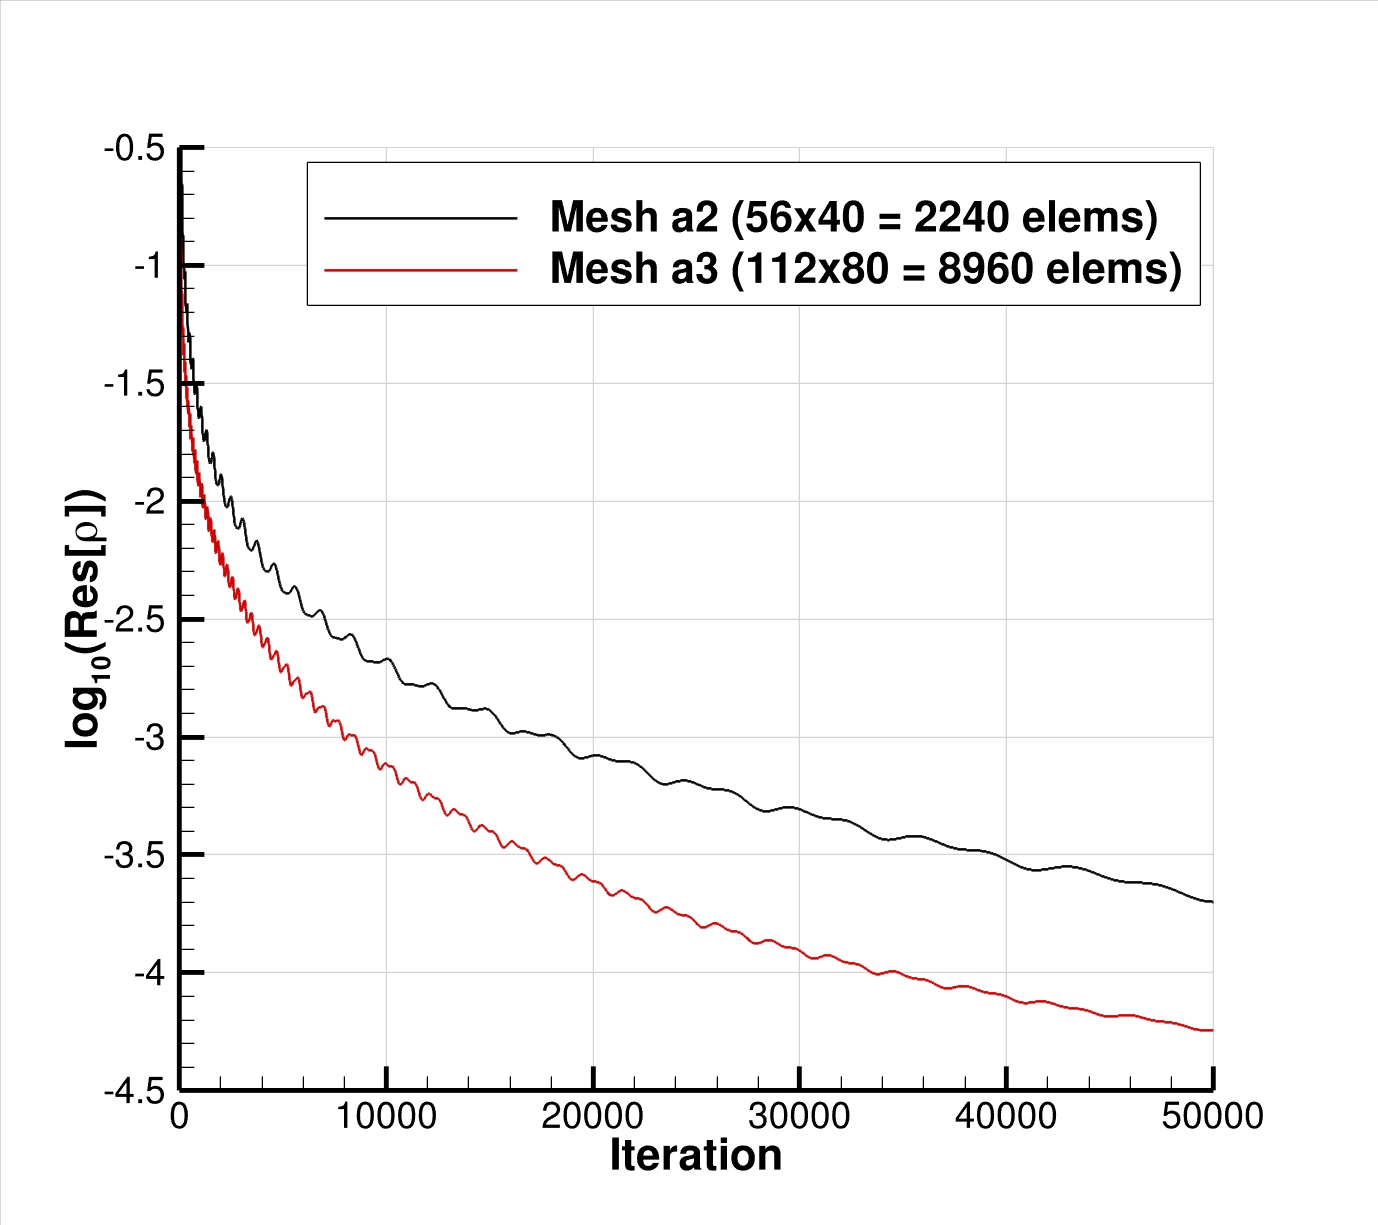
\includegraphics[width = \textwidth]{CompMesh.jpg}
\caption{Convergence comparison (3$^{rd}$ order, finest grids).}
\label{fig:ComparisonOrder}
\end{minipage}
\hfill
\begin{minipage}[t]{0.48\columnwidth}
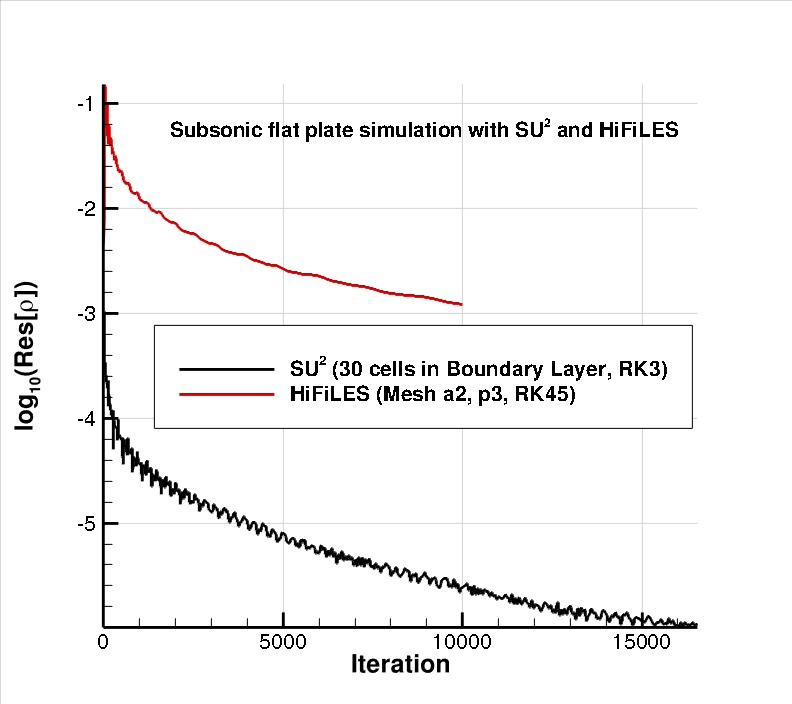
\includegraphics[width = \textwidth] {CompSu2.jpg}
\caption{Comparison of \gls{hf} with SU2 using a similar time integration scheme.}
\label{fig:Comparison_SecondOrder}
\end{minipage}
\end{center}
\end{figure}

To finalize, it is critical to note that the absence of a local time stepping technique in \gls{hf} increases the required number of iterations to obtain a converged solution. However, we have noticed an improvement of the rate of convergence as we refine the grid (see Fig. \ref{fig:ComparisonOrder}). The obtained convergence rate is comparable to a second order numerical code (e.g. SU2~\cite{palacios2013stanford,palacios14}) running using a similar numerical time integration (see Fig.~\ref{fig:Comparison_SecondOrder}).


% Circular cylinder
% !TEX root = ../thesis.tex
\graphicspath{{\aiaadir /figures_cylinder/}}% Set graphics path location

\subsection{Circular Cylinder}

The classic test case of laminar flow past a circular cylinder at low \gls{re} number has also been chosen as a verification and validation case for the 2D \gls{ns} equations in \gls{hf}, and the results are compared to existing experimental data and simulation results~\cite{park1998}. Two separate cases are computed: first, the steady flow past the cylinder at \gls{re}$= 20$, and second, the unsteady flow past the cylinder at \gls{re}$= 100$, where \gls{re} is based upon the diameter of the cylinder. For both cases, \gls{ma} number is set to 0.1 in order to recover nearly incompressible flow for comparisons with the existing incompressible results. The remaining flow conditions are $0\degr$ angle of attack, a constant ratio of specific heats of $1.4$, a Prandtl number of $0.72$, a free-stream temperature of $300K$, and a free-stream dynamic viscosity of $1.853\cdot 10^{-5} Pa \cdot s$ (laminar viscosity varies according to Sutherland's law during the simulation).

The two simulations are performed with third order polynomials on a mesh with $4988$ total elements that contains quadrilateral elements near the body of the cylinder and triangular elements out to the far-field. There is a small refinement box immediately downstream of the cylinder to help resolve features in the wake. The rectangular far-field boundaries are located approximately 30 diameters away from the cylinder in the upstream, upward, and downward directions and 50 diameters away in the downstream direction. A view of the mesh near the cylinder surface is show in Fig.~\ref{cylinder_1}.

\begin{figure}

    \subfloat[Zoom view of the mesh near the cylinder.]{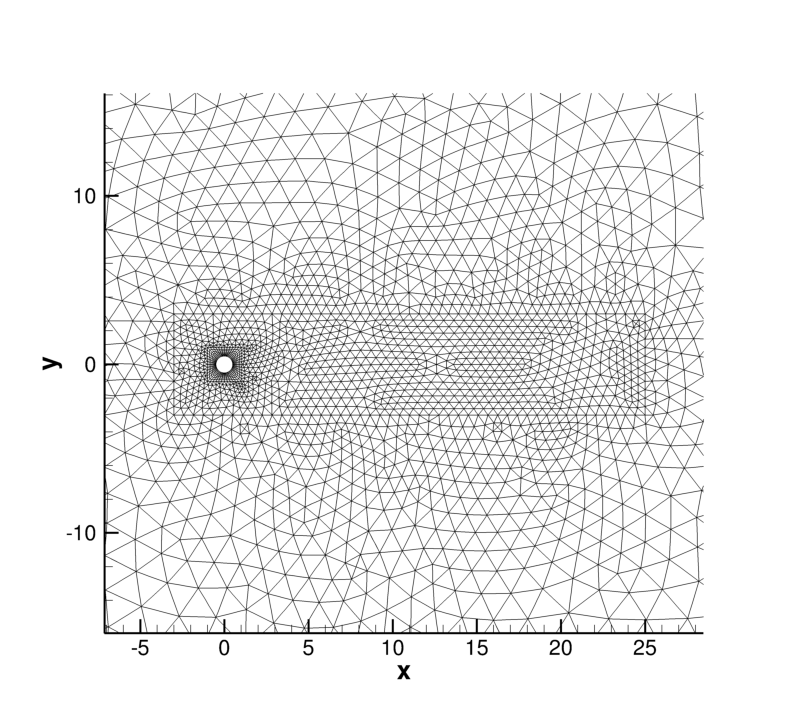
\includegraphics[width = 0.5\textwidth]{cylinder_mesh.png}}
    \subfloat[X-velocity contours and streamlines around the circular cylinder for $Re = 20$.]{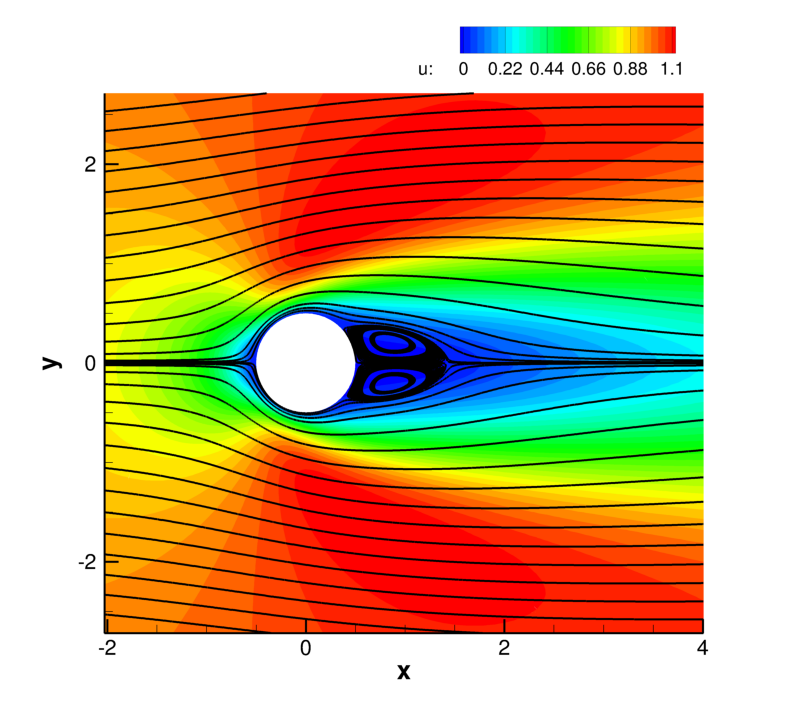
\includegraphics[width = 0.5\textwidth]{cylinder_streamlines.png}}
    
  \caption{The mesh for the circular cylinder simulations along with x-velocity contours for the $Re = 20$ case.}
  \label{cylinder_1}
\end{figure}

The flow around the cylinder for \gls{re}$= 20$ is steady, and it features a large recirculation region behind the cylinder. Fig.~\ref{cylinder_1} presents x-velocity contours around the cylinder along with streamlines. The length of the recirculation region can be determined from the streamlines, and a length of approximately one cylinder diameter agrees well with reported results for \gls{re}$= 20$. The coefficient of drag computed by \gls{hf} is $2.043$, which is close to the value of $2.01$ reported by Park et al.~\cite{park1998} Pressure contours around the cylinder are shown in Fig.~\ref{cylinder_2}.

\begin{figure}

    \subfloat[Pressure contours for the $Re = 20$ case.]{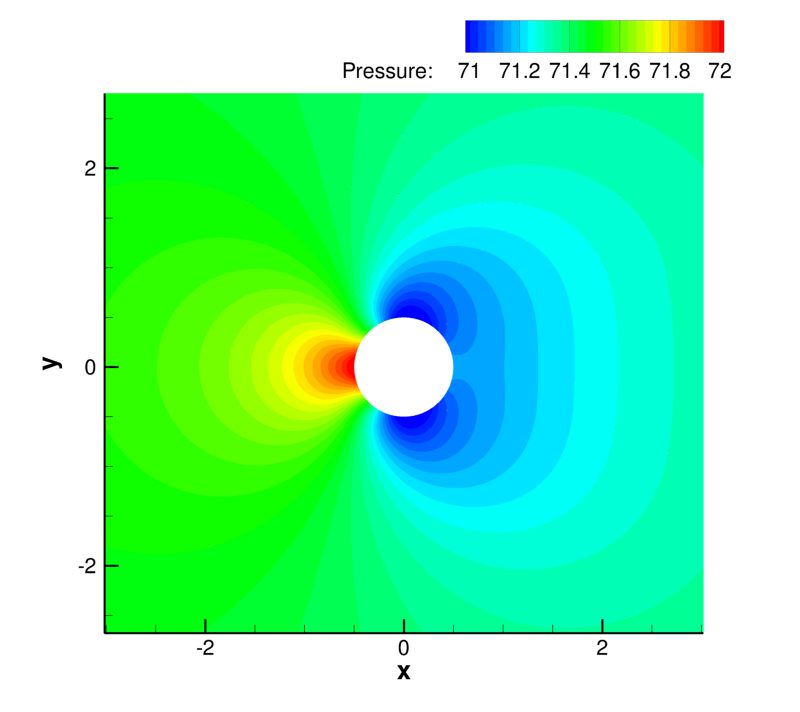
\includegraphics[width = 0.5\textwidth]{cylinder_pressure_re20.png}}
    \subfloat[Pressure contours for the $Re = 100$ case.]{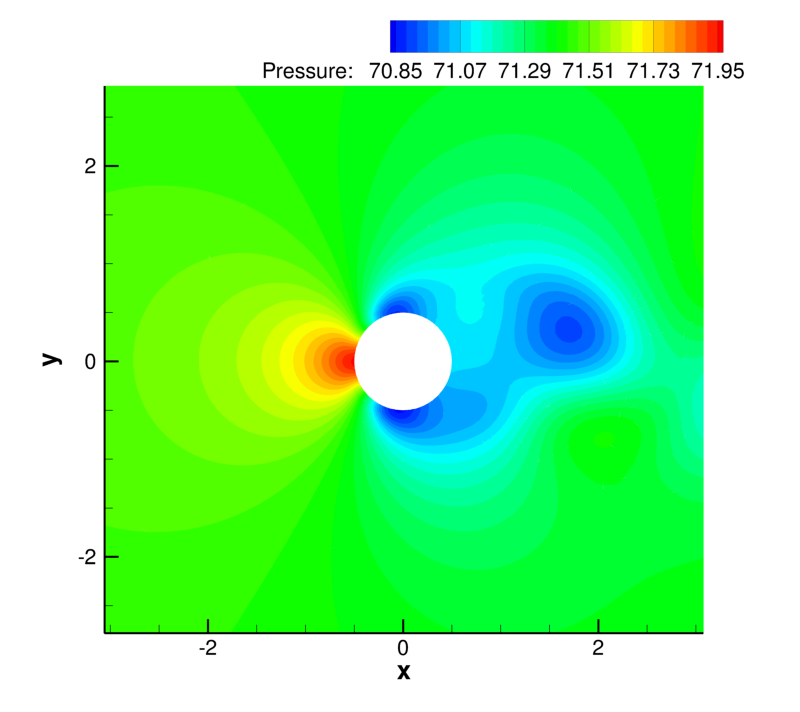
\includegraphics[width = 0.5\textwidth]{cylinder_pressure_re100.png}}

  \caption{Pressure contours for the steady and unsteady (instantaneous) cylinder cases.}
  \label{cylinder_2}
\end{figure}

When \gls{re} is increased to $100$, the flow around the cylinder becomes unsteady and exhibits periodic vortex shedding. This periodic shedding in the wake behind the cylinder can be seen in the instantaneous contours of x-velocity and vorticity in Fig.~\ref{cylinder_3}, and it also results in periodic fluctuations in the force coefficients on the cylinder. \gls{hf} reports an average drag coefficient of $1.339$ with a maximum deviation from this value of $0.0092$, which agree excellently with the values reported by Park et al.~\cite{park1998} of $1.33$ and $0.0091$ for the average $C_d$ and maximum deviation from it, respectively.  Instantaneous pressure contours for the \gls{re}$= 100$ case can be seen in Fig.~\ref{cylinder_2}. The asymmetry that is visible in the pressure contours contributes to the variability in the drag coefficient.

\begin{figure}
    \subfloat[X-velocity contours around the circular cylinder for \gls{re}$= 100$.]{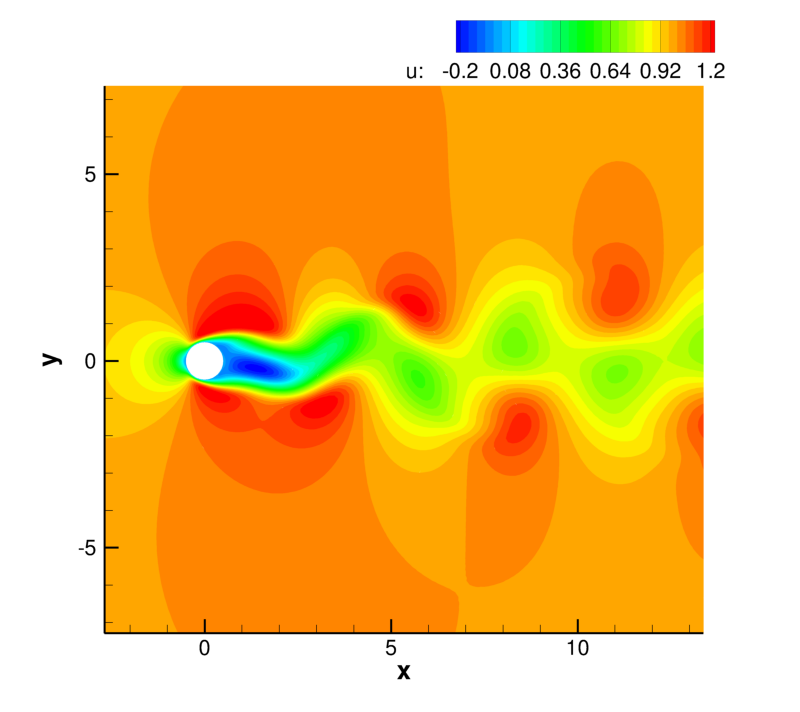
\includegraphics[width = 0.5\textwidth]{cylinder_xvelocity_re100.png}}
    \subfloat[Vorticity contours for the \gls{re}$= 100$ case.]{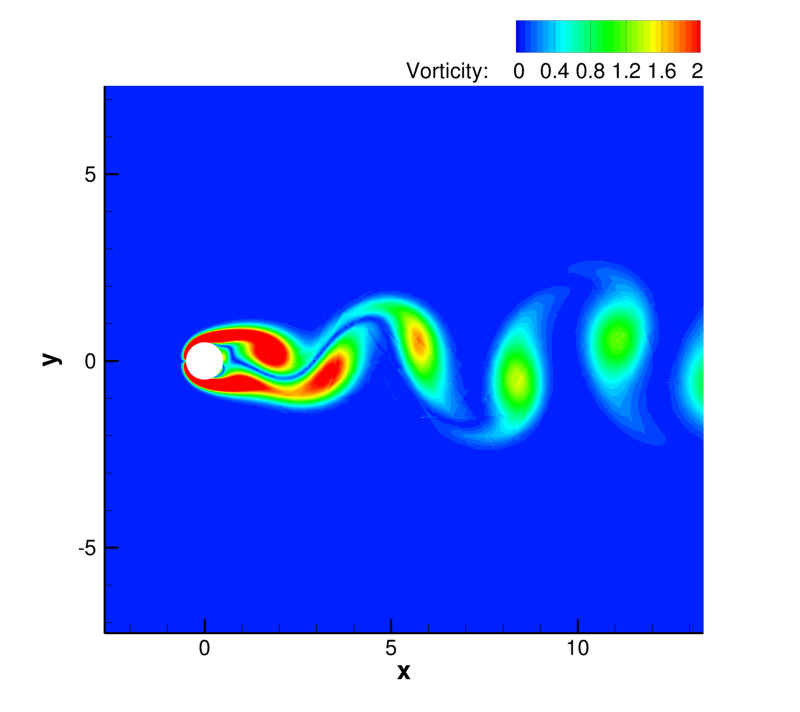
\includegraphics[width = 0.5\textwidth]{cylinder_vorticity_re100.png}}

  \caption{Instantaneous solution contours for the unsteady cylinder case.}
  \label{cylinder_3}
\end{figure}

% SD7003 section
% !TEX root = ../thesis.tex
\graphicspath{{\aiaadir /figures_SD7003/}}% Set graphics path location

\subsection{SD7003 airfoil at 4$\degr$ angle of attack}\label{sd7003airfoil}

Abundant literature documents flow around a SD7003 infinite wing and airfoil. Hence, physical experiments \cite{ol2005comparison,radespiel2007numerical} and numerical simulations \cite{galbraith2008implicit,visbal2009high,castonguay2010simulation,persson2011high,uranga2011implicit} of flow over this geometry can be used to benchmark \gls{hf}.

The simulations on the 2D geometry were performed on a circular domain with a radius of $50c$, where $c$ is the airfoil's cord length, centered at the leading edge of the airfoil. The boundary conditions are characteristic on the outer edge and adiabatic no-slip wall on the airfoil. The Mach number for all simulations was \gls{ma}$= 0.2$. The reported lift and drag coefficients in Table \eqref{table:sdAirfoilForce} correspond to the average of lift and drag coefficients over $13$ periods after the flow reached a pseudo-periodic state. More details are provided by Williams~\cite{williams2013thesis}. 

\begin{table}[htbp]
\centering
\begin{tabular}{ l| l l| l l| l l} 
  
 &  \multicolumn{2}{|c|}{$Re = 10K$}  & \multicolumn{2}{|c|}{$Re = 22K$} & \multicolumn{2}{|c}{$Re = 22K$}  \\ 
 Source & $C_L$ & $C_D$ & $C_L$ & $C_D$ & $C_L$ & $C_D$   \\ 
\hline
 Uranga et al.\cite{uranga2011implicit} & 0.3755 & 0.04978 & 0.6707 & 0.04510 & 0.5730 & 0.02097  \\ 
$c_{dg},\kappa_{dg}$ & 0.3719 & 0.04940 & 0.6722 & 0.04295 & 0.5831 & 0.01975 \\ 
$c_{+},\kappa_{+}$ & 0.3713 & 0.04935 & 0.6655 & 0.04275 & 0.5774 & 0.02005  \\ 
 \end{tabular}
\caption{Time-averaged values of the lift and drag coefficients for the SD7003 airfoil flows with $Re = 10,000, 22,000, 60,000$}
\label{table:sdAirfoilForce} 
 \end{table}

\begin{figure}[htbp]
\centering
\subfloat[Density contours]{
\includegraphics*[trim=0 0 0 0,width=0.48\textwidth]{figure_935a}}
\subfloat[Vorticity contours]{
\includegraphics*[trim=0 0 0 0,width=0.48\textwidth]{figure_935b}}\\

\caption{Density and vorticity contours for the flow with \gls{re}$= 10,000$ around the SD7003 airfoil. $p=2$ on unstructured triangular grid with $N = 25,810$ elements}
\label{sdairfoilre10k}
\end{figure}

\begin{figure}[htbp]
\centering
\subfloat[Density contours]{
\includegraphics*[trim=0 0 0 0,width=0.48\textwidth]{figure_936a}}
\subfloat[Vorticity contours]{
\includegraphics*[trim=0 0 0 0,width=0.48\textwidth]{figure_936b}}\\

\caption{Density and vorticity contours for the flow with \gls{re}$= 22,000$ around the SD7003 airfoil. $p=2$ on unstructured triangular grid with $N = 25,810$ elements}
\label{sdairfoilre22k}
\end{figure}

\begin{figure}[htbp]
\centering
\subfloat[Density contours]{
\includegraphics*[trim=0 0 0 0,width=0.48\textwidth]{figure_937a}}
\subfloat[Vorticity contours]{
\includegraphics*[trim=0 0 0 0,width=0.48\textwidth]{figure_937b}}\\

\caption{Density and vorticity contours for the flow with \gls{re}$= 60,000$ around the SD7003 airfoil. $p=2$ on unstructured triangular grid with $N = 25,810$ elements}
\label{sdairfoilre60k}
\end{figure}

The average lift and drag coefficients are in close agreement with the results by Uranga el. al~\cite{uranga2011implicit}. The density contours in Figures~\eqref{sdairfoilre10k},\eqref{sdairfoilre22k}, and \eqref{sdairfoilre60k} show that vortical structures are captured for a reasonable distance away from the airfoil despite the fact that elements are coarser away from the airfoil.


\newpage

\subsection{SD7003 wing section at 4$\degr$ angle of attack}
To validate \gls{hf}'s performance in 3D simulations, we extrude the SD7003 geometry from Section\eqref{sd7003airfoil} by $0.2c$ in the $z$-direction and apply periodic boundary conditions at $z=0$ and $z=0.2c$. Table \eqref{table:sdWingForce} shows the time-averaged lift and drag coefficients.


\begin{table}[htbp]
\centering
\begin{tabular}{ l| l l| l l| l l} 
  
 &  \multicolumn{2}{|c|}{$Re = 10K$}  \\ 
 Source & $C_L$ & $C_D$    \\ 
\hline
 Uranga et al.\cite{uranga2011implicit} & 0.3743 & 0.04967   \\ 
$c_{dg},\kappa_{dg}$ & 0.3466 & 0.04908  \\ 
$c_{+},\kappa_{+}$ & 0.3454 & 0.04903 \\ 
 \end{tabular}
\caption{Time-averaged values of the lift and drag coefficients for the SD7003 wing-section in a flow with $Re = 10,000$}
\label{table:sdWingForce} 
 \end{table}


\begin{figure}[htbp]
\centering
\subfloat[Density contours]{
\includegraphics*[trim=0 0 0 0,width=0.48\textwidth]{figure_939a}}
\subfloat[Vorticity contours]{
\includegraphics*[trim=0 0 0 0,width=0.48\textwidth]{figure_939b}}\\

\caption{Density and vorticity isosurfaces colored by Mach number for the flow with $Re = 10,000$ around the SD7003 wing-section. $p=3$ on unstructured tetrahedral grid with $N = 711,332$ elements}
\label{sdwingre10k}
\end{figure}

It is worth noting that the vortical structures are preserved better than in the 2D case. Table \eqref{table:sdWingForce} demonstrates that \gls{hf} provides average lift and drag coefficient estimates in close agreement with experiments.



% Taylor-Green Vortex
% !TEX root = ../thesis.tex
\graphicspath{{\aiaadir /figures_taylorgreen/}}% Set graphics path location

\subsection{Taylor-Green Vortex at \gls{re} = 1,600}

The \gls{tgv} is a simple test of the resolution of the small scales of a turbulent flow by a numerical method.
The compressible \gls{tgv} at \gls{re}$=1600$ was one of the benchmark problems in the 1st and 2nd International Workshops on High-Order \gls{cfd} Methods~\cite{wang2013high}.
A reference solution was computed by Debonis~\cite{debonis:13} using a high-order \gls{drp} scheme on a mesh of $512^3$ elements.
The results presented here were obtained by Bull and Jameson using \gls{fr} to recover the fourth-order-accurate \gls{dg} and \gls{sd} schemes in \gls{hf}~\cite{bull2014a,bull2014b}.
We also compare our results to those of Beck and Gassner~\cite{beck:12}, who used a fourth-order filtered \gls{dg} method on a mesh of $64^3$ elements.
From a simple initial condition in a triply-periodic box of dimensions $[0:2\pi]^3$, interactions between vortices cause the flow to develop in a prescribed manner into a mass of elongated vortices across a range of scales.
The initial condition is specified as
%
\begin{eqnarray}\label{tgv}
u(t_0) &&= u_0 \sin (x/L) \cos (y/L) \cos (z/L), \\
v(t_0) &&= -u_0 \cos (x/L) \sin (y/L) \cos (z/L), \\
w(t_0) &&= 0, \\
p(t_0) &&= p_0 + \frac{\rho_0 V^2_0}{16} \left [ \cos \left (\frac{2x}{L} \right ) + \cos \left (\frac{2y}{L} \right ) \right ] \left [ \cos \left (\frac{2z}{L} \right ) + 2 \right ],
\end{eqnarray}
%
where $L = 1$, $u_0 = 1$, $\rho_0 = 1$ and $p_0 = 100$.
\gls{ma} is set to 0.08 (consistent with the initial pressure $p_0$) and the initial temperature is 300K.

Figs.~\ref{dissrate} (a) and (b) show the volume-averaged kinetic energy $\langle k \rangle$  on (a) hexahedral meshes of $16^3$, $32^3$ and $64^3$ elements and (b) tetrahedral meshes (formed by splitting the hexahedral meshes).
The reference solution, labelled as`DRP-512' is plotted for comparison.
Figs.~\ref{dissrate} (c) and (d) show the kinetic energy dissipation rate, given by $\epsilon = -d \langle k \rangle/dt$ versus the reference solution and the results of Beck and Gassner~\cite{beck:12}, labelled as`Beck-DG-64x4'.
On the finest hexahedral and tetrahedral meshes the kinetic energy and dissipation rate predictions match the reference solution, demonstrating that the high-order numerical scheme is able to resolve the important flow dynamics on a relatively coarse mesh.
As a qualitative measure of the resolution of the turbulent flow structures, Figure~\ref{qcrit} shows isosurfaces of the $q$ criterion at four times during the simulation.
The evolution of complex small scale structures is evident.

\begin{figure}[htbp]
\centering
\subfloat[$\langle k \rangle$, hexahedral meshes]{
\includegraphics*[trim=0 0 0 0,width=0.48\textwidth]{tke-SD-hex-mesh}}
\subfloat[$\langle k \rangle$, tetrahedral meshes]{
\includegraphics*[trim=0 0 0 0,width=0.48\textwidth]{tke-SD-tet-mesh.pdf}}\\
\subfloat[$-d \langle k \rangle/dt$, hexahedral meshes]{
\includegraphics*[trim=0 0 0 0,width=0.48\textwidth]{dissrate-SD-hex-mesh.pdf}}
\subfloat[$-d \langle k \rangle/dt$, tetrahedral meshes]{
\includegraphics*[trim=0 0 0 0,width=0.48\textwidth]{dissrate-SD-tet-mesh.pdf}}\\
\caption{\small Taylor-Green vortex results on hexahedral and tetrahedral meshes from Bull and Jameson~\cite{bull2014a}.
(a, b) Evolution of average kinetic energy $\langle k \rangle$; (c, d) dissipation rate $-d \langle k \rangle/dt$.
`SD-$M \times N$' refers to $M^3$ mesh, $N$th-order accurate SD scheme.
(\textbf{- - -}) 4th-order \gls{dg} on $64^3$ mesh~\cite{beck:12}; ($\circ$) \gls{dns}~\cite{debonis:13}.}
\label{dissrate}
\end{figure}

\begin{figure}[htbp]
\centering
\subfloat[$t = 2.5$, $Q=0.5$]{
\includegraphics*[width=0.48\textwidth]{TGV-DG3-hex-64-qcriterion-isosurface-005-velocolor-025s-z-small}}
\subfloat[$t = 5$, $Q=1.5$]{
\includegraphics*[width=0.48\textwidth]{TGV-DG3-hex-64-qcriterion-isosurface-015-velocolor-05s-z-small}}\\
\subfloat[$t = 7.5$, $Q=1.5$]{
\includegraphics*[width=0.48\textwidth]{TGV-DG3-hex-64-qcriterion-isosurface-015-velocolor-075s-z-small}}
\subfloat[$t = 10.75$, $Q=1.5$]{
\includegraphics*[width=0.48\textwidth]{TGV-DG3-hex-64-qcriterion-isosurface-015-velocolor-1075s-z-small}}
\caption{\gls{tgv} solution on the fine mesh using fourth order accurate \gls{dg} method, showing isosurfaces of $q$ criterion colored by velocity magnitude at time $t = 2.5$ to $10.75$ seconds.}
\label{qcrit}
\end{figure}



%Square Cylinder
% !TEX root = ../thesis.tex
\graphicspath{{\aiaadir /figures_squarecylinder/}}% Set graphics path location

\subsection{LES of Flow Over a Square Cylinder at Re = 21,400}\label{sqcyl}

Using the \gls{fr} method to recover the fourth-order accurate \gls{sd} scheme, the flow over a square cylinder of side $D$ in a domain of $21D \times 12D \times 3.2D$ (see Figure \ref{sqcylmesh}) at $Re = 21,400$ and \gls{ma} $0.3$ was simulated, for which \gls{ldv} experimental data is available~\cite{lyn1994,lyn1995}.
A tetrahedral mesh of $87,178$ elements was generated giving a total of $1.74$M \gls{dof} since there are $20$ solution points per element at fourth order accuracy.
Time discretization was by the fourth-order five-stage explicit \gls{rk} scheme.
A total time of $250$ seconds was simulated and time-averaged quantities were calculated over the last $100$ seconds (approx. 5 flow-through periods).
The \gls{wsm} model (see Section \ref{lesmodels}) based on the modal Vandermonde filter~\cite{bull2014a} was used with the Breuer-Rodi three-layer wall model~\cite{breuer1994} within $0.2D$ of the wall.
The computation took around $60$ hours on $7$ GPUs in the lab's own cluster.
Figure \ref{sqcylmesh} shows the computational mesh including all the \gls{dof}.
Figure \ref{sqcylqcrit} shows an isosurface of the $q$-criterion colored by velocity magnitude, illustrating the structures present in the turbulent boundary layer and wake.
Figures \ref{sqcylplots} (a, b) show the normalized mean streamwise and vertical velocity components $\langle u \rangle/u_B$ and $\langle v \rangle/u_B$ respectively along several vertical lines in the wake.
Figures \ref{sqcylplots} (c, d) show the normalized mean Reynolds stress components $\langle u'u' \rangle/u_B^2$ and $\langle u'v' \rangle/u_B^2$ along the same lines.
For comparison, high-order \gls{les} results computed by Lodato and Jameson~\cite{lodato2012b} using the \gls{sd} method and the \gls{wsm} model on a hexahedral mesh of $2.3$M \gls{dof} are plotted.
Mean velocities are accurately predicted although the accuracy is reduced near the cylinder owing to the coarse tetrahedral resolution in the boundary layer.
The Reynolds stresses are less accurately predicted than the mean velocities but are broadly correct.
These results highlight the advantages of using \gls{hf} for \gls{les} of turbulent flows: the ability to obtain good results on coarse meshes and the ability to use unstructured tetrahedral meshes.


\begin{figure}[h] \tt
\centering
\subfloat[geometry]{
\includegraphics*[width=0.61\textwidth]{sqcyl-geom-small}}
\subfloat[boundary layer mesh]{
\includegraphics*[width=0.35\textwidth]{sqcyl-tet-coarse3-blmesh}}
\caption{Square cylinder geometry and tetrahedral boundary layer mesh showing all degrees of freedom}
\label{sqcylmesh}
\end{figure}

\begin{figure}[h] \tt
\centering
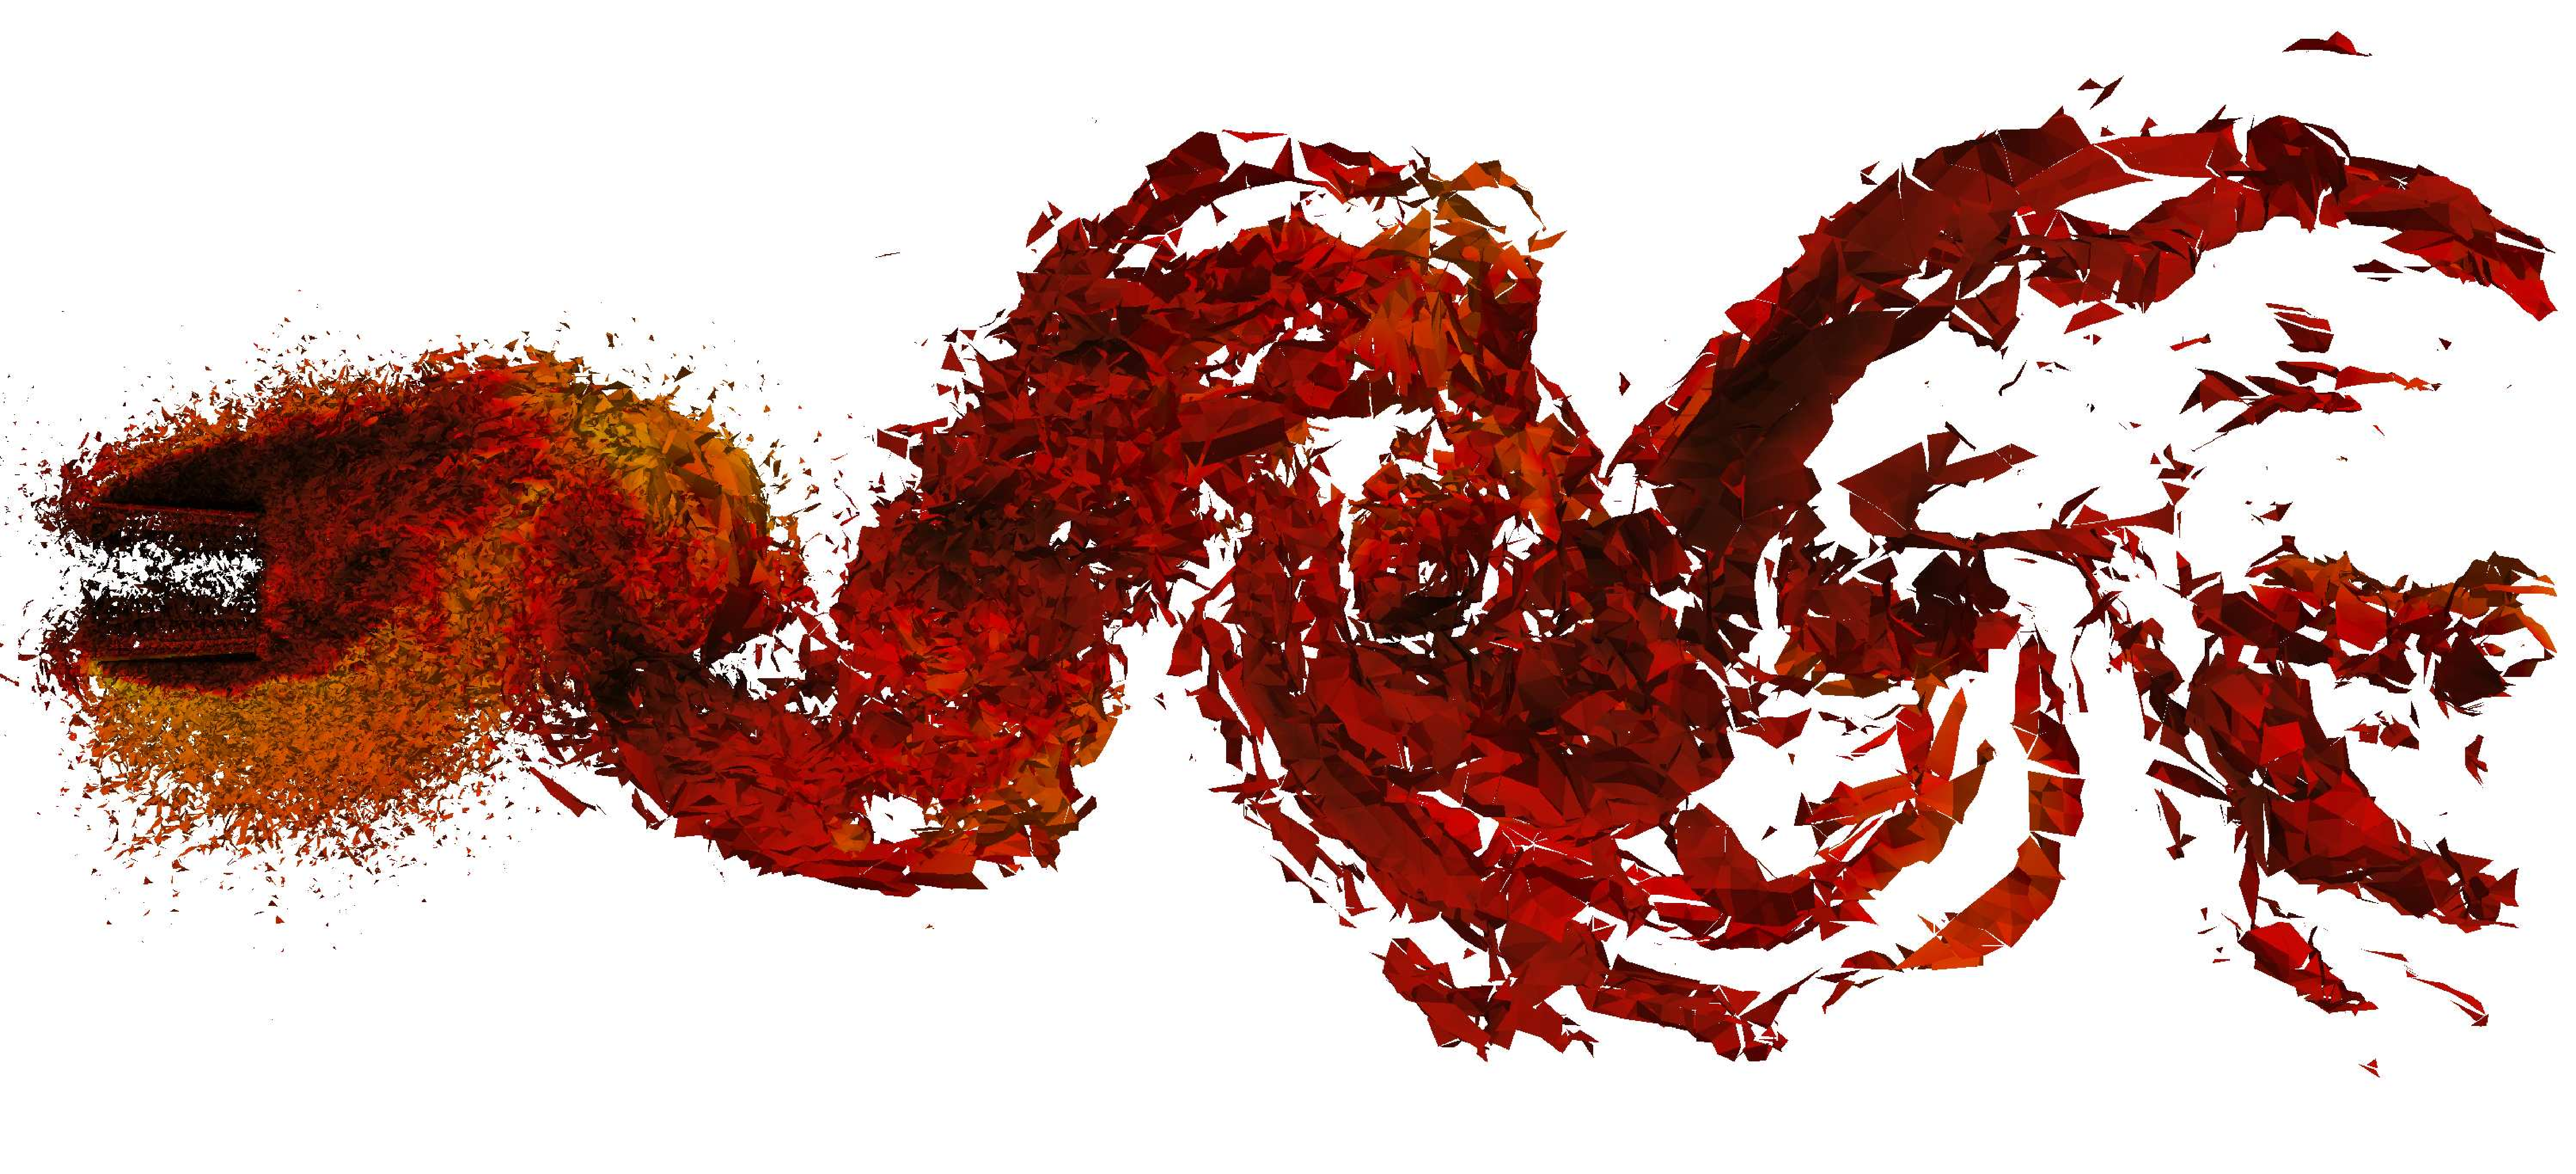
\includegraphics[width=0.9\textwidth]{sqcyl-tet-wsm-newwallfn-coarse3-qcrit-010-velomag.pdf}
\caption{Isosurface of the $q$-criterion colored by velocity magnitude showing the wake behind the square cylinder}
\label{sqcylqcrit}
\end{figure}

\begin{figure}[h]
\centering
\subfloat[Mean streamwise velocity $\langle u \rangle/u_B$]{
\includegraphics*[width=0.8\textwidth]{sqcyl-tet-wsm-newfilt-coarse-fixbc-meanu-vprofile-small.pdf}}\\
\subfloat[Mean vertical velocity $\langle v \rangle/u_B$]{
\includegraphics*[width=0.8\textwidth]{sqcyl-tet-wsm-newfilt-coarse-fixbc-meanv-vprofile-small.pdf}}\\
\subfloat[Mean Reynolds stress $\langle u'u' \rangle/u_B^2$]{
\includegraphics*[width=0.8\textwidth]{sqcyl-tet-wsm-newfilt-coarse-fixbc-meanuu-vprofile-small.pdf}}\\
\subfloat[Mean Reynolds stress $\langle u'v' \rangle/u_B^2$]{
\includegraphics*[width=0.8\textwidth]{sqcyl-tet-wsm-newfilt-coarse-fixbc-meanuv-vprofile-small.pdf}}
\caption{\small (a) Mean streamwise and vertical velocity and mean Reynolds stresses along vertical lines in the wake.
(---) current results, (- - - ) 4th order \gls{sd}+\gls{wsm} on hexahedral mesh by Lodato and Jameson~\cite{lodato2012b}, ($\circ$) \gls{ldv} experiments by Lyn et al.~\cite{lyn1994,lyn1995}.}
\label{sqcylplots}
\end{figure}



% !TEX root = ../thesis.tex
\graphicspath{{\aiaadir /figures_RANS_naca0012/}}% Set graphics path location

\subsection{NACA 0012 airfoil at 0$\degr$ angle of attack, Re = 6 million, Ma = 0.15}
In this section, the NACA 0012 airfoil is used to study the accuracy of the \gls{sa} turbulence model coupled with \gls{fr}. The NACA 0012 is commonly used as a validation case for all turbulence models and a large database of results are available at the NASA Turbulence Modeling Resource website. A $6,539$ element quad/triangle mixed mesh is used with a NACA 0012 airfoil of chord length $1.0$ and a farfield boundary $20$ chord lengths away. The results are compared with CFL3D and experimental results from Gregory \& O'Reilly~\cite{gregory1973low}.

\begin{figure}

    \subfloat[Zoomed view of the mixed element mesh near the NACA 0012 airfoil.]{\includegraphics[width = 0.5\textwidth]{NACA0012_Re6mil_mesh.eps}}
    \subfloat[X-momentum contours near the NACA 0012 airfoil]{\includegraphics[width = 0.5\textwidth]{NACA0012_Re6mil_alp0_momx.eps}}

  \caption{Turbulent flow past a NACA 0012 airfoil at \gls{re} = 6 million, \gls{ma} = 0.15, $\alpha = 0^{\circ}$ using \gls{fr} to recover 4th order accurate \gls{dg} method and the \gls{sa} turbulence model.}
  \label{RANS_naca0012}
\end{figure}

\begin{figure}
\centering
  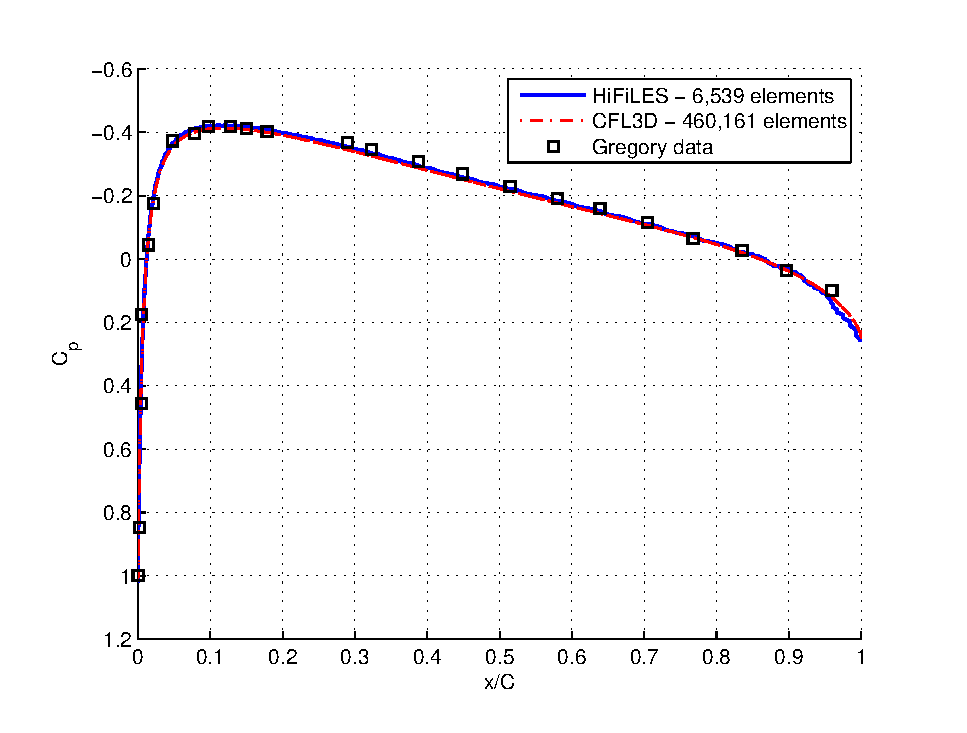
\includegraphics[width=0.48\textwidth]{cp.eps}
  \caption{Pressure coefficient on the NACA 0012 airfoil at \gls{re} = 6 million, \gls{ma} = 0.15, $\alpha = 0^{\circ}$ using \gls{fr} to recover 4th order accurate \gls{dg} method and the \gls{sa} turbulence model.}
  \label{RANS_naca0012_cp}
\end{figure}





% Note that the verification section above now has both V & V
%\section{Validation (Preliminary results)}
\label{sec:validation}
Here we follow some cases from the 2nd High-Order Workshop.

\subsection{Flat Plate}

\subsection{Circular Cylinder}
From David's thesis.



%\subsubsection{Vortex transport by uniform flow (2D)}
%\subsubsection{Transonic Ringleb Flow (2D)}
%\subsubsection{Flow over an Analytical Body of Revolution (3D)}

\subsection{RANS NACA 0012}

\subsection{SD7003 airfoil at 4$\degr$ angle of attack}
From David's thesis\cite{williams2013thesis}
\subsection{SD7003 wing section at 4$\degr$ angle of attack}
From David's thesis.
%\subsubsection{Laminar Flow around a Delta Wing}

\subsection{DNS of the Taylor-Green Vortex at Re = 1,600}

\begin{figure}
\centering
\includegraphics[height=60mm]{./figures/dissrate-hex-mesh-small.pdf} \\
\caption{LES of Tyalor-Green Vortex at Re=1,600\cite{bull2013a}}
\label{fig:setup}
\end{figure}


\subsection{DNS of Decaying Homogeneous Turbulence}
To be done by Manuel
\subsection{LES of Decaying Homogeneous Turbulence}
To be done by Manuel



\section{Conclusion}
\label{sec:conclusion}

We have suggested a formulation of \gls{lfs} filters for the stabilization of \gls{ns} solvers for unstructured grids that use a Finite Element Method-based approach to achieve high order spatial discretizations. This includes \gls{dg}, \gls{sd}, Spectral Element, and \gls{fr} methods. The filtering operation can be performed at individual elements and maintains a local stencil by using the element's solution and boundary values. This makes their implementation highly parallelizable.

The filters have been developed with the desired properties shown in Section \ref{sec:lfs_properties}. In essence, the filters have a spectral interpretation and satisfy boundary conditions asymptotically. The computational cost of applying a filtering operation to a single element is two small matrix multiplications. This low cost plus the compact stencil makes the \gls{lfs} filters a good alternative to using artificial dissipation. The main advantage of \gls{lfs} filters over artificial dissipation is that no modification needs to be made to the partial differential equations being solved.

We have shown by implementing the \gls{lfs} filters in \gls{hf} that little to no tuning is necessary to achieve stability in cases where instability is expected: coarse grids, high-\gls{re} flows, high-\gls{ma} flows, and low-\gls{ma} flows. In all cases, the filters preserved the boundary conditions, did not introduce visible flow anomalies, and allowed the flow to develop its natural features. The summary of results can be seen in Table \ref{table:results}.

Because the filter has a physical interpretation, \gls{sgs} modeling could be done with the classical physical arguments. A similar type of filter has been used by Lodato\cite{lodato2014structural} in the \gls{sd} scheme to do \gls{sgs} modeling rather than to stabilize the solution.

The unexpected finding that the filters could bring simulations in very coarse meshes to a pseudo-steady state opens up the possibility of using the \gls{lfs} filters as part of a pre-conditioning strategy or to start flow simulations from conditions more developed than uniform flow.

All algorithms are publicly available in the \gls{hf} \href{https://github.com/HiFiLES/HiFiLES-solver}{repository} under the branch ``\gls{lfs}-filters". The filters have been fully implemented for \gls{gpu}/CPU computations for triangular grids only.

%The results seen in \cite{asthana2014} are very promising, given that a double shock 2D simulation with $9^\text{th}$ order of accuracy are possible. We have recently submitted an article\cite{asthana2014} to JCP showing the promising results. Due to time constraints (the article was submitted on November 12, 2014), we have not produced results different to those in the article, but expect to have excellent results in the final version.
%

\prefacesection{Acknowledgments}

Mentorship by Peter Vincent, Patrice Castonguay, and David Williams was essential for my involvement in the intellectually stimulating topic of high order methods. David's tenacity, talent, and example helped me keep the passion for modeling and simulation alight. The work of Guido Lodato served as an inspiration for many of the topics of this thesis. Jonathan Bull's application of high order methods to turbulent flows served as guidance for the selection of capabilities that I would like to see in a Navier-Stokes solver.

Prof. Antony Jameson provided me with an invaluable environment of intellectual freedom framed by his sharing of pioneering ideas and insightful recommendations. His mastery of numerical analysis and crispness of communication are traits I shall strive to emulate.

Feedback and questions by Prof. Juan Alonso and Prof. Charbel Farhat have helped me contextualize the contributions in this dissertation in the larger scopes of Aerospace Engineering and Computational Fluid Dynamics. Comments by Prof. Parviz Moin and Prof. Brian Cantwell have encouraged my desire to apply the numerical methods discussed here to simulations relevant to flow physics studies.

Friendship and comradeship with Abhishek Sheshadri, Kartikey Asthana, Jerry Watkins II, Josh Romero, Jacob Crabill, and David Manosalvas made it enjoyable working in the Aerospace Computing Laboratory. I relied on their knowledge and eagerness to help to move past theoretical and implementation hurdles.

I am grateful for the support for this work provided by the Air Force Office of Scientific Research under grant \# FA9550-14-1-0186, monitored by Dr. Fariba Fahroo, and the Aeronautics and Astronautics Departmental Fellowship.

\bibliographystyle{aiaa}

\bibliography{references}

 \end{document}


